\chapter{Trabalhos relacionados}\label{cap:introducao}

Giovanni \citeonline[p.~117]{mori_analysing_2015} define a improvisação de códigos em relação à Música, Imagens em Movimento, Dança ou Tecelagem. É importante esclarecer que essa definição denota a aplicação em qualquer outra área, não apenas como metáfora, mas como técnica para gerenciar o fluxo criativo:

\begin{citacao}
\traducao{\emph{Live coding} é uma técnica artística de improvisação. Pode ser empregada em muitos contextos diferentes de performance: dança, música, imagens em movimento e mesmo tecelagem. Eu concentrei minha atenção no lado musical, que parece ser o mais proeminente.}{Live coding is an improvisatory artistic technique. It can be employed in many different performative contexts: dance, music, moving images and even weaving. I have concentrated my attention on the music side, which seems to be the most prominent.}
\end{citacao}

O problema desta definição é que ela não contempla uma classe puramente técnica da improvisação de códigos, como por exemplo os registros audiovisuais de um tutorial de como escrever um aplicativo \emph{web}\disponivelem{https://www.youtube.com/watch?v=dHtyDron5ik}. No entanto, a premissa da pesquisa é, assim como Mori, situar a improvisação de códigos do ponto de vista musical. Descartamos uma discussão específica sobre imagens em movimento para evitar cair em uma digressão infinita, já que este é outro campo proeminente; mas uma menção será feita em relação ao contexto musical. A discussão sobre tecelagem \ver{sec:tecelagem} contextualiza a história da computação com a prática artística investigada. Além disso, dois improvisadores-programadores chave para a prática, Alex McLean e Dave Griffths, serão apresentados. O primeiro é a Música Eletrônica para Dançar \footnote{\cfcite{hillegonda_dj_2013}.} \ver{sec:algorave}, e o segundo nega o som como resultado da improvisação de códigos \ver{sec:coreografia}. Adiante, a característica musical da improvisações de códigos será explorada do ponto de vista histórico \ver{sec:musica}. Por último, será discutido um conjunto de regras práticas que emergiram durante uma disputa acadêmica. Isto é, a partir de uma problematização feita por \citeonline{schloss_dilemma_2003}, sobre o papel cênico (e visual) do músico que carrega um computador no palco de performance, uma resposta conjunta de McLean, Griffths, Amy Alexander, Adrian Ward, Fredrik Olofsson, Julian Rohrhuber e Nick Collins, \cite{ward_live_2004}, possibilitou a proliferação de idéias e a estruturação de um programa de investigação científica próprio para a improvisação de códigos \ver{sec:laptoptoplap}.

\section{Tecelagem}\label{sec:tecelagem}

Contextualizar a atividade têxtil é uma forma de criar uma imagem mental, de como funciona o processo de computação. Seria possível usar a imagem de um ábaco. Mas essa última imagem não considera potenciais leitores de um programa de pesquisa que inclui investigadores na área de Moda (como é o caso do Programa de Pós Graduação em Artes, Cultura e Linguagens da Universidade Federal de Juiz de Fora). Não aprofundaremos o assunto de Moda, mas sim buscamos ilustrar um código de computador. Nas palavras de \citeonline{griffths_weave2_2015},

\begin{citacao}
 \traducao{Um dos potenciais da tecelagem que eu fiquei mais interessado é a capacidade de demonstrar fundamentos de \emph{softwares} por fios -- parcialmente tornar a natureza física da computação auto-evidente, mas também como uma maneira de modelar novas formas de aprender e a entender o que são os computadores.}{One of the potentials of weaving I’m most interested in is being able to demonstrate fundamentals of software in threads – partly to make the physical nature of computation self evident, but also as a way of designing new ways of learning and understanding what computers are.}
\end{citacao}

Buscamos demonstrar na próxima seção esta natureza física da computação. Através de retrospecto na história da computação irá auxiliar na inclusão da tecelagem na definição de Mori.

\subsection{Charles Babbage e Joseph-Marie Jacquard}

Os computadores atuais são máquinas desenvolvidas com base no modelo teórico elaborado por Alan Turing (1912-1954). Uma representação simplista considera uma fita abstrata de tamanho variável (o quanto for necessário), dividida em células, cada uma com um alfabeto finito. Cada alfabeto possui uma quantidade de símbolos de representação finita. Um cabeçote leitor desta fita lê as instruções escritas em cada célula, e depois passa para a próxima célula. Um registrador de estados desta fita, memoriza qual foi a última operação realizada na última célula executada. Uma tabela de ações indicará novas instruções, que serão escritas nesta fita.

 Um modelo anterior ao de Turing foi elaborado por Charles Babbage (1791 -- 1871), \emph{a máquina analítica},  entre 1834 e 1836, revisado em 1837. Sua construção ocorreu após um colapso na construção de sua \emph{máquina diferencial}. O projeto não vingou, mas a partir de 1838, Babbage se envolveu com a exploração intelectual dos conceitos elaborados, para otimizar o projeto e reduzir seu custo de construção. Uma sequência de seminários em Turin (1840) resultou em uma publicação sobre a máquina analítica, em francês, escrita por um cientista italiano (L.F. Menebrea). A Condessa de Lovelace (Ada Augusta Byron King), traduziu, sob supervisão de Babbage, esta publicação para o inglês. Historicamente, os primeiros programas de computador (para serem executados na máquina analítica) foram escritos ambos por Ada e Babbage. O primeiro programa escrito era dedicado ao cálculo de uma sequência numérica conhecida como \emph{Números de Bernoulli} \footnote{Allan G. Broomley, \emph{Charles Babbage’s Analytical Engine, 1838}. Disponível em \url{http://athena.union.edu/~hemmendd/Courses/cs80/an-engine.pdf}}. Apenas uma parte da máquina foi construída antes da morte de Babbage\disponivelem{http://www.sciencemuseum.org.uk/objects/computing_and_data_processing/1878-3.aspx}.

Segundo \citeonline[p.14--21]{McLean2011}, o mecanismo do projeto de Babbage é inspirado na máquina de tear de Joseph-Marie Jacquard (1752 -- 1834). A principal contribuição da invenção, para a computação, foi um sistema que consiste em um cabeçote leitor de cartões perfurados. Na máquina de tear de Jacquard, a organização dos furos indicam, até hoje, uma rotina têxtil \ver{fig:jacquard}. Já no computador mecânico de Babbage, o cartão perfurado indicava estados binários que conduzem ao cálculo numérico:

\begin{citacao}
\traducao{A indústria têxtil vislumbrou a primeira máquina programável de ampla utilização: a cabeça de tear Jacquard, uma tecnologia ainda usada. Longas tiras de cartão são alimentados na cabeça de tear Jacquard, que lê padrões perfurados no cartão para guiar a intrincada padronização de tecidos. O cabeçote Jacquard não computa, mas foi admirado por Charles Babbage, inspirando o trabalho na sua máquina analítica mecânica, a primeira concepção de um computador universal programável. Embora Babbage não tenha obtido sucesso em construir a máquina analítica, seu projeto inclui um mecanismo de entrada de cartão similar ao cabeçote Jacquard, mas com  padrões perfurados descrevendo cálculos abstratos ao invés de fios têxteis.}{
The textile industry saw the first programmable machine to reach wide use: the head of the Jacquard loom, a technology still used today. Long strips of card are fed into the Jacquard head, which reads patterns punched into the card to guide intricate patterning of weaves. The Jacquard head does not itself compute, but was much admired by Charles Babbage, inspiring work on his mechanical analytical engine (Essinger, 2004), the first conception of a programmable universal computer. Although Babbage did not succeed in building the analytical engine, his design includes a similar card input mechanism to the Jacquard head, but with punched patterns describing abstract calculations rather than textile weaves.
}
\end{citacao}

%\begin{figure}[!h]
%  \centering
%  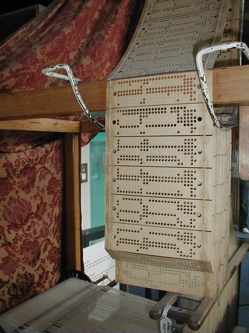
\includegraphics[scale=0.82]{imagens/Jacquard.jpg}
%  \caption{Cartões perfurados da máquina de tear Jacquard. \textbf{Fonte}: wikimedia.org }
%  \label{fig:jacquard}
%\end{figure} 

\subsection{Weavecoding}\label{sec:weavecoding}

Se até hoje o mesmo sistema de Jacquard é utilizado para materializar imagens mentais de formas geométricas, como improvisadores de códigos elaboram uma \emph{estratégia transversal} \ver{sec:tidal}, de transformar a imagem mental destas formas geométricas em códigos, e de códigos para o resultado desejado? De outra forma, como é realizada uma improvisação de códigos audio visuais, musicais e têxteis? Exemplificamos o caso com um grupo que criou o conceito \emph{weavecoding}. Sua definição será dada conforme apresentamos o grupo \emph{Weaving codes}\disponivelem{http://kairotic.org/about/}; ilustramos uma investigação informal, um encontro no Foam Kernow\disponivelem{http://fo.am/kernow/}.

O grupo \emph{Weaving codes} foi formado para  investigar \traducao{padrões a partir das perspectivas de tecelagem e música, e através do desenvolvimento de uma linguagem de computador e código para descrever a construção de tecidos}{We pursue these questions in the Weaving Codes- Coding Weaves project, by investigating patterns from the perspectives of weaving and music, and by developing a computer language and code for describing the construction of weaves}. É formado por membros da Universidades de Leeds, Nottingham Trent, Cambridge, Aberdeen, Copenhague; um museu (\emph{Albert Museum}), uma rede de laboratórios transdisciplinares (FoAM Kernow ); o Centro Dinamarquês para Pesquisa Têxtil, e Escola Robert Schumman de Música e Mídia de  Düsseldorf. 

Uma pequena digressão: dois membros deste grupo, Alex McLean e Dave Griffths, são praticantes e organizadores de improvisações de código como artistas-programadores. A principal contribuição dos autores foi uma heurística da improvisação de códigos, \emph{Lubeck04}, mais conhecido como \traducao{Mostre-nos suas telas}{Show Us Your Screens}, dentro de um manifesto publicado como \traducao{Programação de Algoritmo Ao vivo e Organização Temporária para sua Promoção}{Live Algorithm Programming and Temporary Organization for its Promotion} \cite{ward_live_2004}. Este tema será discutido adiante \ver{sec:showusyourscreens}.

Do manifesto à codificação têxtil, \citeonline{griffths_weave2_2015} apresenta um interessante exemplo. A partir de quatro tarefas fundamentais (rotinas), descritas no Exemplo \autoref{ex:weaving}, é possível elaborar um padrão como o apresentado na \autoref{fig:weaving}. A primeira rotina é \emph{repeat}, uma repetição de ações por contagem $[$\emph{loop}$]$; a segunda é \emph{twist}, ou dar a volta em determinados pontos; a terceira,  \emph{weave-forward}, tecer à frente do ponto; e a quarta, \emph{weave-back}, tecer atrás do ponto . Do lado direito da imagem (ver p.~\pageref{fig:weaving}), é simbolizado o ``código criptografado de tecido'', ou as operações fundamentais para um determinado padrão têxtil. Do lado esquerdo, seu resultado-padrão, uma textura de losangos e zigue-zagues.  

\begin{example}{Um código-fonte que gera um tecido semelhante à \autoref{fig:weaving}.}
\label{ex:weaving}

\begin{minted}[fontsize=\footnotesize]{cl}
(twist 3 4 5 14 15 16)
(weave-forward 3)
(twist 4 15)
(weave-forward 1)
(twist 4 8 11 15)

(repeat 2
 (weave-back 4)
 (twist 8 11)
 (weave-forward 2)
 (twist 9 10)
 (weave-forward 2)
 (twist 9 10)
 (weave-back 2)
 (twist 9 10)
 (weave-back 2)
 (twist 8 11)
 (weave-forward 4))
\end{minted}
\end{example}

\begin{figure}[!h]
    \centering
    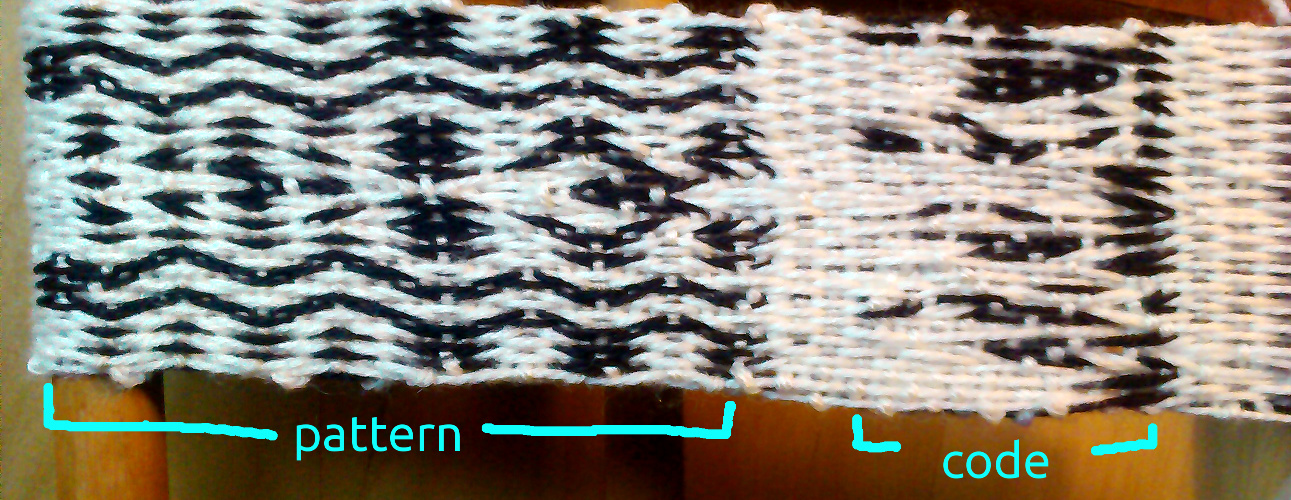
\includegraphics[scale=0.31]{imagens/weaving.jpg}
    \caption{Tecido resultante da prática \emph{Weaving code}. \textbf{Fonte}: \citeonline{griffths_weave2_2015}.}
  \label{fig:weaving}
\end{figure}

Esta experiência de \emph{weavecoding} pode ser aplicada em uma performance. Griffths ilustra uma performance arquetípica da improvisação de códigos: programadores escrevendo enquanto os resultados são projetados em superfícies planas \ver{fig:weavecoding}. Como veremos, é interessante que o que está sendo escrito também seja projetado \cite[p.~129]{McLean2011}, o que não é o caso desta imagem. A tecelagem é programada por meio de um dispositivo tangível \ver{fig:weavecoding2}, uma matriz de botões acopláveis, desenvolvida por Ellen Harlizius-Klück (investigadora da história da matemática, filosofia e tecelagem da Grécia Antiga na Universidade de Copenhague\disponivelem{http://www.saumweberei.de/}) e Alex McLean \ver{fig:weavecoding2}. Imagens em movimento foram projetadas como capturas das atividades têxteis e processadas por Griffths. 

\begin{figure}[h]
  \centering
  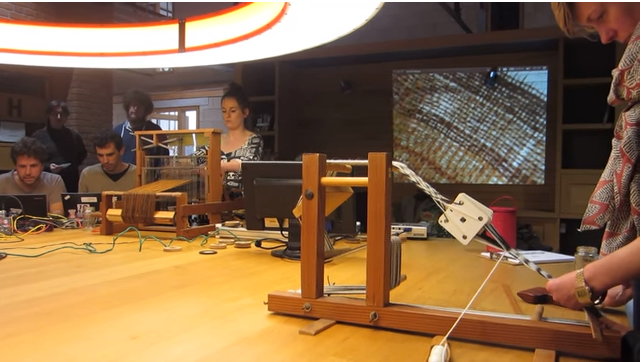
\includegraphics[scale=0.65]{imagens/weaving.png}
  \caption{Performance no Foam Kernow. \textbf{Fonte}: \citeonline{griffths_weave_2015}.}
  \label{fig:weavecoding}
\end{figure}

\begin{figure}[h]
  \centering
  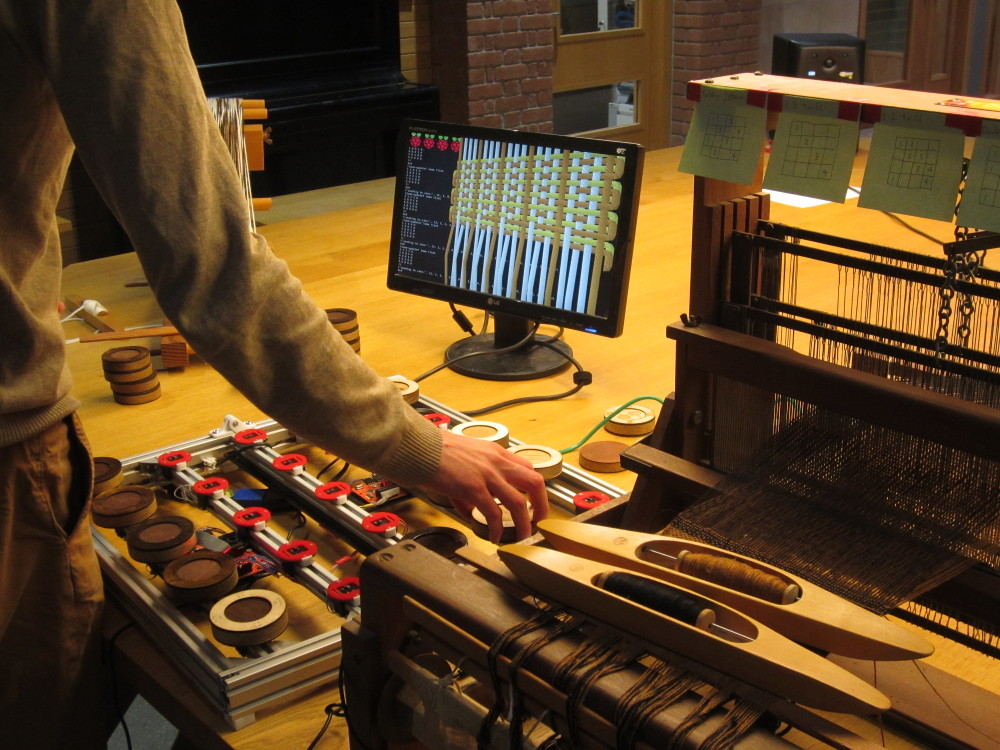
\includegraphics[scale=0.8]{imagens/weavecoding.jpg}
  \caption{ Alex McLean manipulando uma Matriz de botões para tecelagem, conectado a um Raspberry Pi. \textbf{Fonte}: \citeonline{griffths_weave_2015}.}
  \label{fig:weavecoding2}
\end{figure}

\begin{citacao}

\traducao{
Uma das idéias originais era combinar tecelagem e codificação em um cenário de atuação, ambos para fornecer uma forma de tornar a codificação ao vivo mais inclusiva com a tecelagem, e ao mesmo tempo esclarecer os processos de pensamentos digitais envolvolvidos na tecelagem (\ldots) Nossa audiência consistiu de pesquisadores de artesanato, biólogos antropológicos, arquitetos, designers de jogos e tecnólogos -- foi mais do que antecipamos! Alex e eu disponibilizamos alguns códigos de música do \emph{slub} para tecer, e minha parte favorita foi projetar a tecelagem ao vivo.
}{
One of the original ideas we had was to combine weaving and coding in a performance setting, to both provide a way to make livecoding more inclusive with weaving, and at the same time to highlight the digital thought processes involved in weaving. (\ldots) Our audience consisted of craft researchers, anthropological biologists, architects, game designers and technologists -- – so it all went on quite a lot longer than we anticipated! Alex and I provided some slub livecoded music to weave by, and my favourite part was the live weaving projection.
}
\end{citacao}

Esta descrição de Griffths possui uma documentação audiovisual \disponivelem{https://www.youtube.com/watch?v=XrnIVUp9QgM}. É interessante notar que a menção ao grupo \emph{Slub} auxilia a discussão musical, e ao mesmo tempo articula esta seção com a próxima. 

\subsubsection{Slub}

A banda \emph{Slub} começou em 2000, como uma colaboração entre Adrian Ward e Alex McLean. A premissa do duo era utilizar a atividade de programação para realização de uma Música Eletrônica de Dança\footnote{\cfcite{hillegonda_dj_2013}}. Sua primeira reunião foi em 2001, no \emph{Paradiso club} em Amsterdã, durante o festival \emph{Sonic Arts}. Em 2005 Griffths se juntou ao duo durante o festival \emph{Sonar}, o que abriu espaço para o desenvolvimento de uma estética de videogames \cite[p.~138--140]{McLean2011}.

É interessante notar que a improvisação de códigos já era mencionada em documentações de \emph{softwares}, antes do \emph{Slub} ou do manifesto de \citeonline{ward_live_2004}. No entanto, as metodologias de improvisação de códigos são diversas. A utilização de ambientes como \emph{SuperCollider}, \emph{iXiLang}, PureData ou Max/MSP, estão restritas ao contexto de linguagens de domínios específicos\footnote{\emph{Domain Specific Language} ou DSL.}. O então duo \emph{Slub} seguiu o seguinte caminho: a utilização de linguagens de propósito geral\footnote{\emph{General-Purpose Language} ou GPL.}, como Perl, REALBasic e Scheme \ver{sec:impromptu}. Além disso, uma descrição destes sistemas GPLs oferecem a descrição de uma característica interessante. Por exemplo, a justificativa de aceitação de uma música para dançar \ver{sec:algorave} é feita através de uma postura bastante trivial, projetar o que está fazendo no computador; no entanto esta trivialidade não deve ser subestimada, afinal hoje ela é considerada como uma regra heurística. Segundo \citeonline[p.~139]{McLean2011}:

\begin{citacao}
\traducao{Um sistema Slub antigo é descrito em detalhes por \citeonline{collins_generative_2003}. De maneira breve, ele apresentava um sintetizador, um antigo sistema de codificação ao vivo escrito por Ward, e uma série de programas geradores de batidas e linhas de baixo escritos por McLean. Embora o seu principal objetivo era musical, o Slub gostava de ser confrontado com o desafio de serem aceitos como programadores que fazem música. Para este fim, começou projetando suas telas de audiências com uma sobreposição conceitual, entre seu \emph{softwares} artesanais, e a música que  produziam com seu uso.}{An early Slub system is described in detail by \citeonline{collins_generative_2003}. In brief it featured a synthesiser and early live coding system written by Ward, and a Number of beat and bass-line generating programs by McLean. Although their primary aim was musical, Slub enjoyed beign faced with the challenge of beign accepted as programmers who make music. To this end they began projecting their screens audiences with the conceptual overlap between their and-crafted software and the music they produced using it.}
\end{citacao}

Em 2004, com a formação do TOPLAP \ver{sec:toplap}, Ward e McLean focaram seus eforços no desenvolvimento de ambientes de improvisação de códigos. É interessante notar que os sistemas elaborados,  são uma mistura de linguagens textuais, \emph{patching} e interfaces gráficas de usuário\footnote{\emph{Graphical User Interfaces} ou GUIs.}: \traducao{O \emph{Slub} controlava sua música usando interface criadas por e para eles mesmos. Eles variam desde os aparentemente convencionais para os abstratos, e das $[$interfaces$]$ gráficas para a inteiramente textuais.}{Slub control their music using user interfaces created by and for themselves. These vary from the apparently conventional to the abstract, and from graphical to entirely textual.}
\cite[p.~323]{collins_generative_2003}. A descrição abaixo detalhada algumas das funções destes programas, bem como um processo de composição por redes que será discutido em outra oportunidade \ver{sec:baiasaofranscisco}:

\begin{citacao}
\traducao{Por detrás das interfaces \emph{slub} residem os processos 'composicionais' ou 'musicais' -- muitos pedaços de códigos separados, escritos como exploração de idéias musicais. Cada pedaço de código descreve um experimento em áreas como matemática combinatorial, progressões de acordes, modelos sonificados para as pessoas dançarem, métricas que sofrem transformações, batidas sincopadas algorítmicas, e outros. (\ldots) Estes processos composicionais enviam mensagens de um para o outro através de uma rede TCP/IP usando um protocolo de linha de comando. As mensagens viajam através de um servidor central, que administra a sincronização temporal entre os processos \emph{Slub}. (\ldots) O protocolo de rede resolve um problema que poderia, de outra forma, ser insolúvel: Adrian e Alex muitas vezes tomam abordagens muito diferentes para fazer música. Contudo eles não tem que argumentar sobre como a música é feita. Porque eles concordaram sobre, e implementaram um protocolo de rede, eles são livres para fazer música do jeito que gostarem, sabendo que seus programas irão sincronizar um com o outro.}{Behind the slub interfaces lie the ‘compositional’ or ‘musical’ processes – many separate pieces of code written as explorations of musical ideas. Each piece of code describes an experiment in such areas as combinatorial mathematics, chordal progressions, sonified models of dancing people, morphing metres, algorithmic breakbeats, and so on. (\ldots) These compositional processes send messages to one another other across a TCP/IP network using a line-based protocol. The messages travel via a central server, which also manages time sync between all the slub processes. (\ldots) The network protocol solves a problem which might otherwise be unsolvable: Adrian and Alex often take very different approaches to making music. However, they don’t have to argue about how the music is made. Because they agreed upon and implemented a network protocol between their programs, they are free to make music however they like, knowing that their programs will synchronise with each other.} 
\end{citacao}

\section{Dança}\label{sec:danca}

A Dança é ilustrada de duas maneiras. A primeira é dança como fim de uma improvisação musical. O código recodificado, e projetado de maneira semelhante ao \emph{Slub}, corre o risco de ser a atração principal. O segundo caso foge do escopo sonoro; uma coreógrafa codifica apenas a orientação espacial de uma bailarina, resultando em uma sensação de quietude sonora. É uma posição que diverge da maioria dos trabalhos apresentados, mas é pouco discutido no âmbito musical. 

\subsection{Algorave}\label{sec:algorave}

A compositora colombiana Alexandra Cárdenas, em entrevista com \citeonline{chesire_algorave_2013}, cita Nick Collins e Alex McLean como os criadores do termo \emph{algorave} (\emph{algorithm} $+$ \emph{rave} ). Surgiu durante uma \emph{gig} (um termo utilizado no início do \emph{jazz} para caracterizar um trabalho temporário). Após sintonizarem em uma estação de rádio, decidiram codificar uma música semelhante:

\begin{citacao}
\traducao{
Algorave 'comecou como uma piada', de acordo com Alex McLean, um pesquisador de música computacional e um dos três de uma banda chamada \emph{Slub}, que têm improvisado códigos por 13 anos. Ele veio com um termo enquanto conduzia uma \emph{gig} em Nottingham com seu amigo Nick Collins (que tocava ``datapop'' sob o nome Sick Lincoln) no final de 2011. 'Nós sintonizamos em uma estação pirata tocando \emph{happy hardcore}, e nós pensamos que seria bom programar alguma música \emph{rave}.' Deste então, McLean organizou oito \emph{algoraves} informais no mundo.
}
{
Algorave "started as a joke", according to Alex McLean, a computer-music researcher and one-third of a band called Slub that's been live coding for 13 years. He came up with the term while driving to a gig in Nottingham with his friend Nick Collins (who plays "datapop" under the name Sick Lincoln) in late 2011. "We tuned into a pirate station playing happy hardcore, and we thought it would be good to program some rave music." Since then, McLean has organised eight informal algoraves around the world. 
}
\end{citacao}

Em seu artigo ``Algorave: Live Performance of Algorithmic Electronic Dance Music'', \citeonline[p.~356]{collins_algorave_2014} sustentam que as estruturas das práticas do \emph{algorave} são anteriores à improvisação de códigos, e já era utilizado na Música Eletrônica para Dançar. O que mantêm a relação entre os dois é a prática de projeção do código \ver{sec:laptoptoplap}.

\begin{citacao}
\traducao{
\emph{Algorave} não é sustentado exclusivamente por \emph{live coders}, mas estes têm mantido uma forte presença em todos os eventos até agora. É assim talvez porque a tradição do \emph{live coding} de projetar telas motiva todo o esforço; onde algoritmos não estão visíveis por períodos de tempo durante uma \emph{algorave}, se corre o risco das coisas parecerem muito como um evento de música eletrônica padrão.
}
{Algorave is not exclusively a preserve of live coders, but they have maintained a strong presence at every event thus far. This is perhaps because the live coding tradition of projecting screens help motivates the whole endeavour; where algorithms are not made visible for periods during an algorave, we run the risk of things feeling much like a standard electronic music event.}

\end{citacao}

Focando no aspecto histórico, \citeauthoronline{collins_algorave_2014} descrevem uma sequência de eventos (desenvolvimentos de \emph{softwares} e apresentações). Em 1992, Charles Ames disponibiliza o \emph{Cybernetic Composer}, \traducao{um \emph{software} com um sistema baseado em Inteligência Artificial que compõe musica em uma variedade de estilos populares.}{an AI based software system that composes music in a variety of popular styles. Disponível em \url{http://www.kurzweilai.net/charles-ames}}. Em 1994, o duo \emph{Koan}, formado pelos DJs Daniel Roeth e William Grey, realizam adaptações para entretenimento com base no \emph{ambient music} de Brian \citeonline{eno_music_1978}. \emph{Aphex Twin} (Richard David James) cria em 1997 o termo \emph{live club algorithm}. Em 1999, o protocolo para edição audiovisual ao vivo \emph{bbcut} \cite{collins_bbcut_2003} é incluído nos \emph{opcodes} do \emph{CSound}\footnote{Disponível em \url{https://csound.github.io/}.}, e do \emph{Supercollider}\disponivelem{http://supercollider.sourceforge.net/audiocode-examples/}. Em 2000 o então duo \emph{Slub}, realizam performances, autodenominadas \emph{generative techno}, com abordagem \emph{gabba}. Em 2001 é identificada a utilização de redes neurais para composição de padrões semelhantes ao \emph{drum'n'bass}. Em 2004 é fundado o TOPLAP em uma casa noturna de Hamburgo.

Ilustramos três casos recentes, onde a improvisação de códigos é uma técnica utilizada. Junto com a improvisação de códigos, são utilizados um instrumento eletrônico, voz, e um instrumento elétrico. O inglês Canute, o mexicano Mico Rex e a colombiana residente na Alemanha, Alexandra Cárdenas.

\begin{figure}[!h]
  \centering
  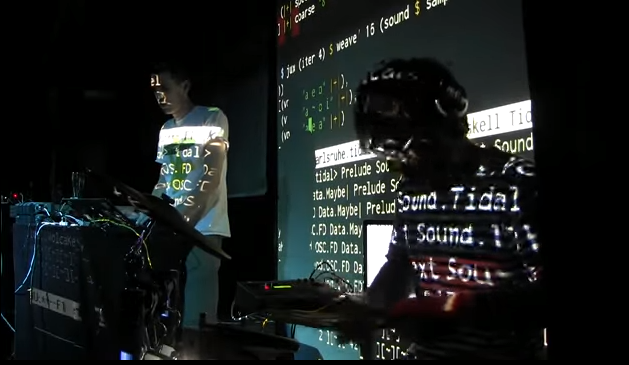
\includegraphics[scale=0.71]{imagens/canute.png}
  \caption{Performance do duo Canute (Karlesruhe, 2015) \textbf{Fonte}: \citeonline{mclean_canute_2015}.}
  \label{fig:canute}
\end{figure}

O registro audiovisual do duo Canute, Matthew Yee-King (bateria eletrônica) e Alex McLean (\emph{laptop}), reforça o arquétipo comentado anteriormente (p.~\pageref{fig:weaving}). A recomendação ``Obscurantismo é perigoso, mostre-nos suas telas''\label{sec:showusyourscreens} é seguida à risca. Categorizações musicais como \emph{club} e \emph{chordpunch} são mencionados na descrição do vídeo. É curioso notar que, em alguns momentos do vídeo, certas modificações nos códigos causam uma perturbação brusca em sistema de ritmos, percebido através do fluxo musical. Em alguns momentos Yee-King mantem o fluxo, mas em outros o instante musical codificado leva um curto período de tempo para ser sincronizado, o que leva Yee-King a se confundir, e por um breve instante, escutar o código e aí retornar à execução. Essa quebra no fluxo musical pode atrapalhar o fluxo de movimentos do corpo. No final deste capítulo, discutimos que este pode não ser \emph{a priori} um erro do instrumentista, mas sim um problema entre o não-esforço cênico de McLean e o esforço de Yee-King. Esta questão cênica será mencionada na \autoref{sec:showusyourscreens}.

\begin{figure}[h]
  \centering
  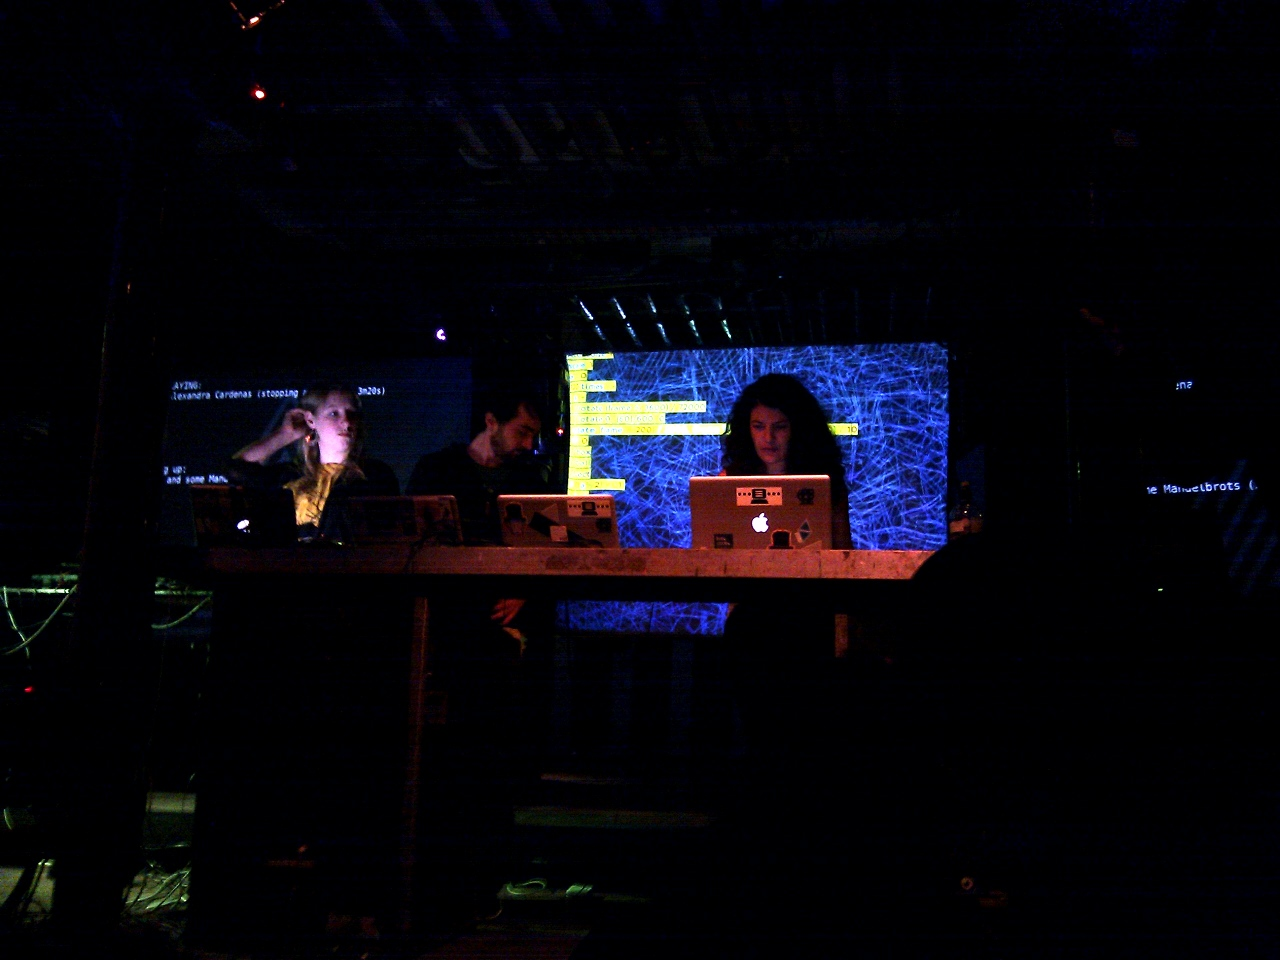
\includegraphics[scale=0.3]{imagens/cardenas.jpg}
  \caption{Performance do duo Mico Rex (Londres, 2013) \textbf{Fonte}: \citeonline{griffths_algorave_2013}.}
  \label{fig:cardenas}
\end{figure}

\begin{figure}[!h]
  \centering
  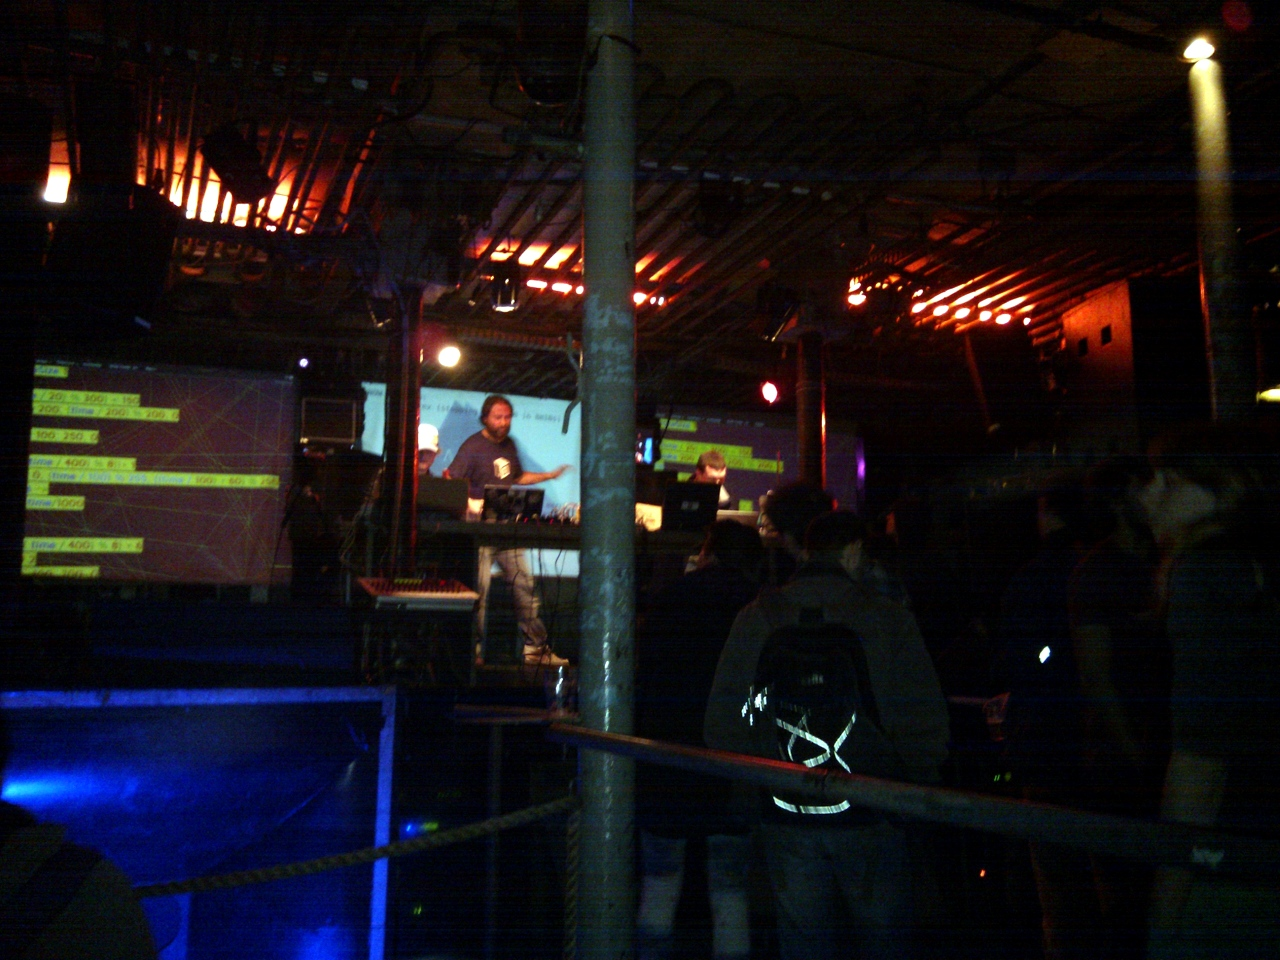
\includegraphics[scale=0.3]{imagens/algorave.jpg}
  \caption{Performance do duo Mico Rex (Londres, 2013) \textbf{Fonte}: \citeonline{griffths_algorave_2013}.}
  \label{fig:micorex}
\end{figure}

Griffiths registra uma \emph{rave} na embarcação  MS Stubnitz, em Canary Wharf, Londres, em 2013. Cárdenas e Ernesto Romero/Jorge Ramírez -- Mico Rex, \ver{fig:micorex} -- tocam neste evento. Encontramos um registro audiovisual de curta duração da apresentação do duo Mico Rex\disponivelem{https://vimeo.com/65309754}, mas não de Cárdenas. Exemplos sonoros específicos estão disponíveis nas redes sociais \emph{SoundCloud} e \emph{Vimeo} \footnote{\url{https://soundcloud.com/tiemposdelruido} e \url{https://soundcloud.com/micorex/}.}. Notas descritivas nestes perfis especificam instrumentos e linguagens de programação, mas não o processo criativo. MicoRex utiliza voz e \emph{programação} ao vivo com o ambiente de programação \emph{SuperCollider}\ver{sec:supercollider}. Entre as categorizações musicais mencionadas, \emph{electro-pop}, \emph{8bits/glitch}, \emph{electro}, \emph{punk}, \emph{bolero} e \emph{breakz}. Cárdenas realiza suas performances com guitarra e programação ao vivo com o \emph{SuperCollider}. É interessante que Cárdenas menciona a utilização de\emph{techno}, \emph{dubstep} e \emph{noise} -- além de distorções, utliliza um misto de instrumento expandido (objetos diversos jogados, friccionados, apoiados na guitarra) e retroalimentação de sinais com níveis saturados.  

\subsection{Coreografia}\label{sec:coreografia}

O segundo exemplo de um contexto de dança é projeto de Kate Sichio, \emph{Hacking the Body}/\emph{Hacking Choreography} \cite{sichio_hacking_2004}. Dois exemplos (\emph{Hacking Coreography 2.0} \emph{v.01} e \emph{v.02}), mais um, \emph{Hacking The Body 2.0}, serão colocados em discussão para ilustrar a ausência do som na improvisação de códigos (o que não significa necessariamente sensação de quietude sonora).

Para Sichio, a relação entre codificação e a dança é parte de um trabalho contínuo entre notação de coreografias e a improvisação. Diferente das indicações estritas de um pentagrama musical, a partitura de dança ofereçe mais um guia para os movimentos do corpo. Isto é, a partitura de dança é mais próxima do código de computador do que a partitura musical tradicional. A assimilação de algoritmos computacionais na Dança, ou \emph{Sensibilidades Computacionais}, é mencionada por \citeonline[p.~31]{sichio_hacking_2004}, através de \citeonline[cap.~1, p.~3]{downie_choreography_2005}. São dispositivos metafóricos, elaborados por coreógrafos como Merce Cunningham, Trisha Brown, Bill T. Jones, e William Forsythe: \traducao{mecanismos de generalização e abstração, representação da coreografia e dança como computação}{mechanisms of generalization and abstraction, choreography as representation, dance as computation} \cite[cap.~1, p.~2--4]{downie_choreography_2005}:

\begin{citacao}
\traducao{Esta sensibilidade computacional é presente em dois níveis em um trabalho destes coreógrafos. Primeiramente, em seus processos coreográficos -- os sistemas, métodos, e notação através dos quais os coreógrafos criam a dança. Segundo, no trabalho ele mesmo, finalizado, que aparece no palco e é interpretado pelo observador. As primeiras invenções e proclamoções dde Cunningham -- a democracia do espaço do palco, e a redescoberta do que está atrás do dançarino como ponto de origem do movimento -- pode ser interpretado como generalizações do tipo; qualquer ponto do palco é a ``frente'', e conectado por um conjunto de articulações pode ser pensado como um membro. O que eram constantes, uma vez especificados em uma descrição rígida, se tornam variáveis em uma estrutura generativa.}{This computational sensibility is present at two levels in the work of these choreographers. Firstly, in their choreographic processes — the systems, methods, and notations through which the choreographers create the dance. Secondly, in the finished work itself, as it appears on stage and as it is interpreted by the viewer. (\ldots) Cunningham’s earliest inventions and proclamations — the democracy of the stage space, and the rediscovery of the dancer’s back as a point of origin of motion — can be interpreted as generalizations of a kind; any point of a stage can be a “front”, and any connected set of joints can be thought of as a limb. What were once specified constants in a rigid description become variables in in a generative framework.}
\end{citacao}

O projeto \emph{Hacking the Body}/\emph{Hacking Choreography} será descrito a partir de \emph{Hacking Choreography beta v.01}, que vai até \emph{Hacking Choreography beta v.04}, apresentados no \emph{Lincoln Performing Arts Centre} em janeiro de 2012 e o último, em maio de 2013 no \emph{Gnarl Festival} (Inglaterra). A experiência parte de uma primeira versão (\emph{v.01}), um \emph{hackeamento} de uma Partitura de Eventos do artista Alison Knowles (mais especificamente a peça de performance \#8, de 1965) . Por exemplo, a partitura é projetada atrás do espaço de performance. Executantes lêem a partitura \ver{code:knowles},

\begin{example}{Partitura original de Alison Knowles (1965)}
\scriptsize
Divida uma variedade de objetos em dois grupos. 
Cada grupo é rotulado com "tudo". 
Estes grupos podem incluir diversas pessoas. 
Existe uma terceira divisão do palco, objetos vazios, rotulados com "nada". 
Cada um dos objetos é "alguma coisa". 
Um executante combina e ativa os objetos das seguintes maneiras para qualquer duração desejada de tempo :
\begin{itemize}
\item "alguma coisa" com "tudo"
\item "alguma coisa" com "nada"
\item "alguma coisa" com "alguma coisa"
\item "tudo" com "tudo"
\item "tudo" com "nada"
\item "nada" com "nada"
\end{itemize}
\end{example}\label{code:knowles}

e seguem com pedaços de papéis, segundo a orientação dada:

\begin{citacao}
\traducao{Depois que a partitura foi completada, contudo, ela foi \emph{hackeada}. Isso significa que o executante tenta de alguma forma contornar as instruções originais. Isto foi feito sem preparações prévias e a audiência assistiu isso se desdobrar enquanto era realizada. Nesta primeira performance, o papel e os rótulos foram rasgados para criar novas palavras e categorias (\ldots) Então ao invés de ``nada''$[$Nothing$]$, foram formados dois grupos, ``não''$[$No$]$ e ``coisa''$[$Thing$]$.}{After the score was completed, however, it was then hacked. This meant that the performer had to try to somehow circumvent the original instructions. This was done with no previous preparation and the audience watched this unfold as the piece was performed.In this first performance, the paper and the labels were torn up to create new words and categories (\ldots). So instead of “Nothing” there were two new groups, “No” and “Thing.”}
\end{citacao}

A segunda experiência, \emph{Hacking Coreography v.02}, é inspirada na proposta de definir termos e associar uma ordem ao termo (como no exemplo anterior). Mas dessa vez, as orientações são escritas como um híbrido de texto discursivo, legível por um executante, e de código de computador em linguagem Java. Isto é, ele não é executável por um computador para resultar em sons, mas por um humano para resultar em movimentos. Isto é, uma seção \emph{set up} define as posições iniciais, \emph{movement} define os tipos de movimentos que serão executados por intérpretes, e \emph{coreography} define uma estrutura de fluxo destes movimentos, e por último, uma ordem de execuções .É interessante notar que Sichio aponta para um outro \emph{hackeamento} da partitura: a utilização de números dificultou a leitura dos intérpretes. Uma alteração na função \emph{coreography} foi feita pelos próprios intérpretes, para alterar a notação numérica por uma descrição textual da ação. 

\begin{example}{Exemplo de um hackeamento de partitura de movimentos}
\begin{minted}[fontsize=\scriptsize]{java}
/Dance/
set up()
{
dance a centre, right
dance b centre, left
}

movement()
{
move1 (dance a = rotate) (dance b = jump)
move2 (dance a = brush) (dance b = lie down)
move3 (dance a = push) (dance b = run)
move4 (dance a = step) (dance b = kneel)
}

coreography()
{
if (dancer a = rotate right 180)
then both jump = 2 feet to 1
if (dancer b = travels)
then brush = right foot
}

run(){
move1
move4
move4
move1
move2
move3
move1
move2
move3
move4
}

/hack/
{
if (dancer a = kneel)
dancer a = kneel
if (dancer a = rotate)
dancer b = rotate opposite direction 
}
\end{minted}
\end{example}



O \emph{Hacking The Body 2.0}, ou \emph{HTB2.0} (2015)\disponivelem{https://www.youtube.com/watch?v=iOAffWTBVE0} é uma performance mais formal. Se caracteriza por uma apresentação em um evento internacional, com um o palco-arena que reforça a hierarquia ator-público (o palco fica aproximadamente na linha da cabeça do espectador). A coreógrafa está sentada ao lado direito do palco, visível, mas debaixo de uma penumbra. Já a dançarina, cuja vestimenta branca equilibra com uma iluminação frontal e estática, expressa uma face de seriedade\ver{fig:iclcdanca}. A performance, segundo  A coreografia segue uma partitura de movimentos corporais.  Mas esta partitura não é visual (o registro não é feito em papel), o resultado da apresentação não são movimentos corporais pré-definidos, e tão pouco existe um acompanhamento musical. Esta partitura é um correlato acústico do tato, codificada por uma coreógrafa. Afastada de uma bailarina, controla a direção dos movimentos corpóreos da performance:

\begin{citacao}
\traducao{Esta peça é uma exploração de eletrônica codificada ao vivo e movimentos improvisados. Uma dançarina veste uma peça de atuadores hápticos. Estes atuadores são programados em tempo-real via OSC\footnote{N.A.: ``\emph{Open Sound Control} é um protocolo de comunicação entre computadores, sintetizadores sonoros e outros dispositivos multimídia que são otimizados para as modernas tecnologias de rede''. Disponível em \url{http://opensoundcontrol.org/introduction-osc}} para 'zunir' sobre os lados direito e esquerdo da dançarina para indicar qual lado do corpo a dançarina deve mover. A partitura é codificada ao vivo pela coreógrafa enquanto a dançarina responde por uma retroalimentação háptica. Esta peça explora o \emph{live coding} de corpos, e movimento como saída, ao invés de saídas sonoras ou visuais como encontrado em muitas execuções de \emph{live coding}
}{
This dance piece is an exploration of live coded electronics and improvisational movement. A dancer wears a custom garment of haptic actuators. These actuators are programmed real-time via OSC to 'buzz' on the right and left sides of the dancer to indicate which side of the body the dancer will move. The score is being live coded by choreographer while the dancer is responding to the haptic feedback. This piece explores live coding of bodies and movement as output rather than a sonic or visual output as found in many live coding performances. \emph{Disponivel em \url{http://iclc.livecodenetwork.org/performances.html}}.
}
\end{citacao}

\begin{figure}[!h]
  \centering
  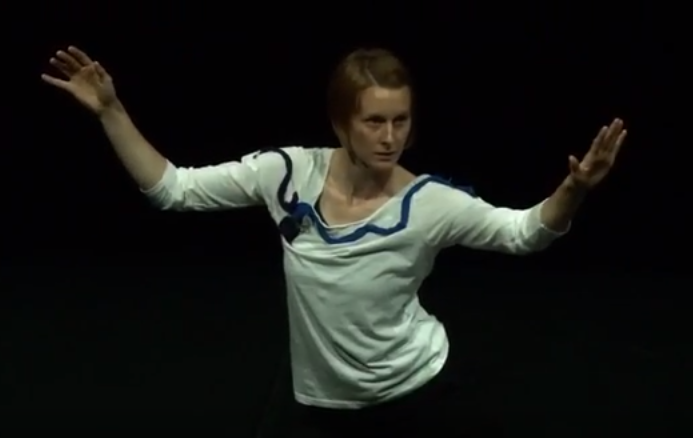
\includegraphics[scale=0.6]{imagens/iclcdanca.png}
  \caption{Dançarina (anônima) controlada por Kate Sicchio (2015) através de uma codificação improvisada. \textbf{Fonte}: \url{https://www.youtube.com/watch?v=uAq4BAbvRS4}.}
  \label{fig:iclcdanca}
\end{figure}

É interessante notar uma sensação de quietude sonora \footnote{\cfcite{koellreutter_wu-li:_1990,el_haouli_abertura_2011}}na performance, mas pouco discutida do ponto de vista musical. Como aponta a própria coreógrafa, a maioria das performances de improviso de códigos segue o seguinte procedimento: o código é criado, e um som, uma nota, uma imagem ou um vídeo são gerados, combinados, transformados de maneira contínua. Mas o padrão é a realização audiovisual. Mesmo em algumas performances de dança pesquisadas (e que não foram mencionadas neste documento), a dança e a projeção audiovisual se suportam. A criatividade deste trabalho toca um conceito técnico fundamental da computação: qual é o \emph{dispositivo de entrada e de saída} praticado nas improvisações de códigos? Sicchio responde que o corpo já é um dispositivo de entrada e saída de interações sociais e pode ser controlado por outro humano através de comandos de rede. A sensação de quietude é presente não por questões musicais, mas é definido por uma prática de dança.


\section{Música computacional}\label{sec:musica}

Apresentamos dois interessantes exemplos realizados com o \emph{SuperCollider}. O primeiro é um ambiente de programação recorrente no ambiente acadêmico \ver{sec:concerto}. A segunda será uma performance telepresencial \ver{sec:telepresenca}. Por último, apresentamos uma perspectiva histórica da improvisação de códigos \ver{sec:protohistoria}. Isto é, \citeonline{ward_live_2004} mencionam uma proto-história da improvisação de códigos, ou eventos artísticos relacionados à \emph{Live Computer Music}.


\subsection{Música de concerto e audiovisual}\label{sec:concerto}

\emph{screenBashing} de Magno Caliman (ver \autoref{fig:screenbashing}) foi realizado durante o XIII ENCUN\footnote{Encontro Nacional de Compositores Universitários em Campinas-SP no ano de 2015.}. Será útil para exemplificar uma \traducao{(\ldots) performance de \emph{livecoding} arquetípica $[$que$]$ envolve programadores escrevendo códigos no palco, com suas telas projetadas para a audiência.}{The archetypal live coding performance involves programmers writing code on stage, with their screens projected for an audience.}\cite[p.~1]{mclean_tidal_2010}. No entanto, a tradução ``improviso de códigos'' como correlato de \emph{livecoding}, bem como a própria definição de \citeonline{mori_analysing_205} \ver{cap:introducao}, se tornam problemáticas em \emph{screenBashing}. Segundo o próprio compositor\footnote{Comunicação pessoal}:

\begin{citacao}
Não acho totalmente adequado considerar como puramente um improviso. Existe, desde a concepção da peça, uma intenção de composição ali. Composição no sentido de agenciamento de materiais \emph{a priori}, entende? Claro, existe um nível de abertura ali com relação a, por exemplo, os caracteres que eu uso no loop, ou nos valores dos parâmetros do \emph{Supercollider} (\ldots). Existem sessões formais ali que, se eu tocar a peça novamente, vão se manter. Daí vc já percebe uma determinação no âmbito macro da coisa também. Em uma situação limite, eu consigo imaginar até uma partitura (de execução) para essa peça, que permitiria que outra pessoa tocasse, sem ver o video da minha performance, e chegasse em resultados bastante similares. Então eu vejo uma série de características aí que diferem de um improviso, onde se espera que uma parte grande do processo de tomada de decisão seja feita no momento da performance. Claro que essa distinção entre composição/peça/determinação e performance/improviso/indeterminação é complexa e a discussão foge totalmente do escopo do seu trabalho. Mas só para atentar para esse detalhe. acredito que se imaginarmos um \emph{continuum}, uma linha onde de um lado vc tem uma improvisação totalmente livre (impossível de se alcançar, claro) e do outro uma composição 100\% determinada (tão impossível quanto), acredito que \emph{screenBashing} está posicionada mais à direita...
\end{citacao}


A performance consiste no seguinte: Caliman senta-se ao computador, lateralmente à tela de projeção, com uma iluminação de penumbra. O projetor expõe o estado atual de seu \emph{laptop}, que apresenta um editor de texto. O executante começa a programar em linguagem C (ver exemplo abaixo). Um pequeno laço iterativo (\emph{for loop}) repete caracteres diversos, improvisados. Assim que termina de escrever, abre um console (ou terminal nos sistemas operacionais Unix) e compila o programa -- a compilação é um processo no qual a representação textual humana, definida pela ANSI\disponivelem{http://www.ansi.org/}, é convertida códigos binários. Este processo não demora, e o programa é executado. O resultado é uma sequência de caracteres de texto como texturas visuais. É importante lembrar que Caliman utiliza um recurso técnico do sistema operacional, que torna o terminal semi-transparente, o que permite sobreposições de texturas. A transformação da textura visual é levada a cabo através da modificação do argumento de entrada da função \verb|printf| (caracteres entre aspas).

\begin{figure}[!h]
  \centering
  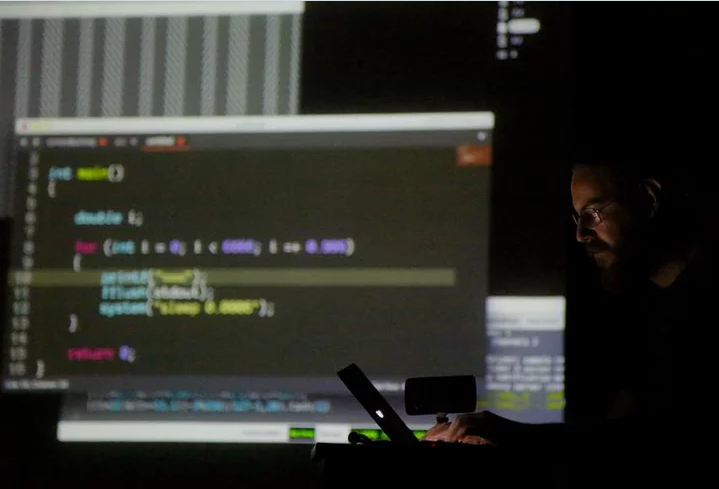
\includegraphics[scale=0.5]{imagens/screenbashing.png}
  \caption{Performance de \emph{screenBashing}. \textbf{Fonte}: \url{https://vimeo.com/148626379}.}
  \label{fig:screenbashing}
\end{figure}

\begin{example}{Algoritmo inicial de Magno calimann}
\begin{minted}{c}
# include <stdio.h>

int main()
{
  double i;
  
  for (int i=0; i<; i < 6666; i=+0.999)
  {
      printf("\\\\    //  \\");
      fflush(stdout)
      system("sleep 0.0006")
  }
}
\end{minted}

Execução:

\begin{minted}{bash}
# gcc - compilador
# a.c - arquivo em linguagem c
# -o  - escreve o resultado em um outro arquivo
# a   - arquivo binario alvo
gcc a.c -o a
\end{minted}

Este código gera algumas mensagens classificadas como \emph{warnings}, ou erros de lógica, que não atrapalham a execução do código em pequenos programas. 

\begin{minted}{bash}
magno.c: In function 'main':
magno.c:7:12: error: conflicting types for 'i'
\end{minted}

Resultado:

\begin{minted}{bash}
\\\\    //  \\\\\\    //  \\\\\\    //  \\\\\\    //  \\\\\\    //
  \\\\\\    //  \\\\\\    //  \\\\\\    //  \\\\\\    //  \\\\\\  
  //  \\\\\\    //  \\\\\\    //  \\\\\\    //  \\\\\\    //  \\\\
\\    //  \\\\\\    //  \\\\\\    //  \\\\\\    //  \\\\\\    //  
\\\\\\    //  \\\\\\    //  \\\\\\    //  \\\\\\    //  \\\\\\    
//  \\\\\\    //  \\\\\\    //  \\\\\\    //  \\\\\\    //  \\\\\\
    //  \\\\\\    //  \\\\\\    //  \\\\\\    //  \\\\\\    //  \\\
\\\    //  \\\\\\    //  \\\\\\    //  \\\\\\    //  \\\\\\    //  
\\\\\\    //  \\\\\\    //  \\\\\\    //  \\\\\\    //  \\\\\\    /
/  \\\\\\    //  \\\\\\    //  \\\\\\    //  \\\\\\    //  \\\\\\  
  //  \\\\\\    //  \\\\\\    //  \\\\\\    //  \\\\\\    //  \\\\\
\    //  \\\\\\    //  \\\\\\    //  \\\\\\    //  \\\\\\    //  \\
\\\\    //  \\\\\\    //  \\\\\\    //  \\\\\\    //  \\\\\    /
\end{minted}
\end{example}

Uma análise atenta do algoritmo visual pode ultrapassar os aspectos técnicos e apontar ideologias. Este é um campo com poucos estudos e não será feito neste trabalho. Limitamo-nos a comentar a experiência auditiva, e visual, contrapondo-a com a declaração do compositor. Para o autor deste texto, a repetição dos algarismos seis e nove, seria uma menção direta (e espelhada) de signos do \emph{black metal} abstrato. Ou seja, um processo sincrético entre a imagem, o código (que de certa forma, faz parte da imagem) e o som (explicado adiante) é notável. No entanto o compositor declara que esta foi uma decisão tomada na hora, como uma piada, embora tenha alguma relação. Mas isso não quer dizer que, para o compositor, a sonoridade se configura como \emph{black metal}. Objetamos que a questão do gênero ultrapassa questões de gosto ou prática sonora, se baseando mais em costumes sociais, como o que se veste, o que se fala, o que se bebe, etc\footnote{\cfcite{janotti_jr._a_2003,sa_se_2009}}. Por outro lado, uma segunda notação mais enxuta e sem erros, permite apontar a questão:

\begin{example}{Correção ao algoritmo de Magno}

O início do código anterior pode ser corrigido. Os novos caracteres foram inseridos por Caliman em 2$'$18$''$:

\begin{minted}{c}
# include <stdio.h>
int main(){
  int i=0;
  for (;;i++){
      printf("=====  ______");
      fflush(stdout);
      // 30 frames por segundo (1/30)
      system("sleep 0.033");
      // 3 frames por segundo (1/3)
      // system("sleep 0.33")
  }
}
\end{minted}

Resultado:

\begin{minted}{bash}
=====  ______=====  ______=====  ______=====  ______=====  ______=====
  ______=====  ______=====  ______=====  ______=====  ______=====  ___
___=====  ______=====  ______=====  ______=====  ______=====  ______==
===  ______=====  ______=====  ______=====  ______=====  ______=====  
______=====  ______=====  ______=====  ______=====  ______=====  _____
_=====  ______=====  ______=====  ______=====  ______=====  ______====
=  ______=====  ______=====  ______=====  ______=====  ______=====  __
____=====  ______=====  ______=====  ______=====  ______=====  ______=

\end{minted}
\end{example}

Os caracteres \verb|\\\\    //  \\| e  \verb|=====  ______|, assim como outros, são sobrepostos. Esse processo ocorre com uma sensação de quietude sonora (ainda assim, este aspecto não é explorado musicalmente, mas essa não é a intenção da música). O improvisador abre códigos preparados no ambiente de programação  \emph{SuperCollider}\disponivelem{https://supercollider.github.io}, que realiza a síntese de texturas sonoras ruidosas. Segundo o compositor, foram \emph{tweets} encontrado na \emph{internet}\disponivelem{https://twitter.com/sc140tweets}. Um novo som ruidoso é adicionado para cada nova textura visual. Este processo, de alternar a codificação da textura visual, e depois executar um programa no \emph{SuperCollider}, é repetido até o fim da peça. A acumulação de sons e caracteres em movimento, cria um contínuo audiovisual que em um momento, as texturas visuais e sonoras entram se tornam um mesmo objeto audiovisual. O processo de compilações e execuções sucessivas exigem cada vez mais e mais do processamento do computador. No auge de saturação visual, sonora e de memória do computador, a improvisação finaliza com um silêncio brusco, decorrente do congelamento do sistema operacional. Essa característica, de pane sistêmica será revista \ver{sec:kuivila}.

\subsection{Telepresença e espaços virtuais}\label{sec:telepresenca}

Uma performance virtual de \emph{live coding} é aquela em que dois ou mais executantes, em endereços diferentes de uma rede de computadores. Isso situa três casos, do qual especificaremos um: i) uma rede local, com computadores diferents, mas com os improvisadores fisicamente próximos; ii) uma rede remota, privada, que comunica um conjunto de pessoas fisicamente distantes; iii) a rede mundial de computadores, onde o navegador se torna o ambiente virtual de criação musical \cite{roberts_web_2013}. Em ambos, a premissa é compartilhar o mesmo código. Podem também compartilhar do mesmo som, mas isso depende da implementação técnica.

O primeiro caso é bastante documentado nas \emph{live coding sessions}, sessões de improvisações que ocorrem em encontros, simpósios e \emph{workshops}, ricamente documentadas\disponivelem{https://supercollider.github.io/archive}.  

Um exemplo do segundo caso é descrito por \citeonline[p.~152--153]{junior_supercopair_2015}. Uma performance telepresencial em 2014, por Ben Swift, Henry Gardner e Andrew Sorensen, realizada \traducao{entre dois intérpretes-programadores localizados na Alemanha e Estados Unidos usando um servidor SSH localizado na Australia}{between two live coders located in Germany and United States using an SSH server located in Australia.}. \citeauthoronline{junior_supercopair_2015} ainda descrevem o desenvilesforço de um ambiente chamado \emph{Supercopair}\disponivelem{https://github.com/deusanyjunior/atom-supercopair}, um ambiente cooperativo de improvisação de códigos, possível através de serviços de computação em nuvem.    

Execuções remotas assíncronas (isto é, entre duas ou mais pessoas, em tempos diferentes) estão sendo exploradas a partir do uso musical de um navegador de \emph{internet}. São realizadas em \emph{apps} como \emph{Gibber} \cite{roberts_gibber:_2012}\disponivelem{http://gibber.mat.ucsb.edu/}, \emph{Wavepot}\disponivelem{http://www.wavepot.com} e \emph{Vivace} \cite{vieira_vivace:_2015}, através da biblioteca \emph{WebAudio API}\disponivelem{https://dvcs.w3.org/hg/audio/raw-file/tip/webaudio/specification.html}. Um \emph{software} na mesma direção foi desenvolvido, uma colaboração entre o autor deste documento e um membro da banca\footnote{\cfcite{lunhani_termpot_2015}}.  

\subsection{Proto-história musical}\label{sec:protohistoria}

Esta seção será dedicada à construção de um espaço conceitual histórico, do ponto de vista musical. Isto é, aqueles exemplos citados como ``proto-históricos'' que possuem alguma similaridade com o conjunto de regras práticas publicadas por \citeauthoronline{ward_live_2004} \ver{sec:laptoptoplap}, cujo objetivo é a criação sonora. 

\citeonline{mori_pietro_2015} descreve um caso prematuro de \emph{live coding} na Itália, com o compositor Pietro Grossi \ver{sec:grossi}. Divergente em algumas das propostas de Max Mathews, sacrificou a questão timbrística para trabalhar na questão performática. As atividades de grupos como \emph{The Hub}, e compositores como Ron Kuivila, no final da década de setenta e anos oitenta, são descritos como como fundamentais para o entendimento histórico do \emph{live coding} em seus aspectos técnicos\ver{sec:baiasaofranscisco}. Um recorte do documento-manifesto ``\emph{Live Algorithm Programming and Temporary Organization for its Promotion}'', de \citeauthoronline{mclean_patterns_2009}, será feita na \autoref{sec:laptoptoplap} para discutir identidade cultural da organização TOPLAP. Na \autoref{sec:showusyourscreens}, ``Show us your screens'', é revisto como o manifesto que define as regras práticas do \emph{live coding}, e a ideologia de projeção de telas.


\subsubsection{Pietro Grossi}\label{sec:grossi}

Embora pouco conhecido no contexto geral da música européia, o compositor Pietro Grossi foi  um dos pioneiros da \emph{Computer Music} Italiana. O pensamento musical que rege seus programas de computador sacrifica questões timbrísticas para concentrar na performance. O primeiro \emph{software} desenvolvido foi o DCMP (\emph{Digital Computer Music Program}) e, segundo \citeonline[p.~126]{mori_pietro_2015}, ao usar este programa,

\begin{citacao}
\traducao{(\ldots) o intéprete era capaz de produzir e reproduzir música em tempo real, digitando alguns comandos específicos e os parâmetros composicionais desejados. O som resultante vinha imediatamente depois da operação de decisão, sem qualquer atraso causado por cálculos. Haviam muitas escolhas de reprodução no programa: era possível salvar na memória do computador peças de músicas pré-existentes, para elaborar qualquer material sonoro no disco rígido, para administrar arquivos musicais e iniciar um processo de composição automático, baseado em algoritmos que trabalham com procedimentos ``pseudo-casuais''. Exsitia também uma abundância de escolhas para mudanças na estrutura da peça. Um dos mais importantes aspectos do trabalho de Grossi foi que todas intervenções eram instantâneas: o operador não tinha que esperar pelo computador terminar todas operações requisitadas, e depois ouvir os resultados. Cálculos de dados e reprodução sonoras eram simultâneos. \textbf{Esta simultaneidade não era comum no campo da \emph{Computer Music} daquele tempo, e Grossi deliberadamente escolheu trabalhar desta forma, perdendo muito no lado da qualidade sonora. Seu desejo era poder escutar os sons resultantes imediatamente}.}{(\ldots) the performer was able to produce and reproduce music in real time by typing some specific commands and the desired composition's parameters. The sound result came out immediately after the operator's decision, without any delay caused by calculations. There were many reproduction choices inscribed in this software: it was possible to save on the computer memory pieces of pre-existing music, to elaborate any sound material in the hard disk, to manage the music archive and to start an automated music composition process based on algorithms that worked with “pseudo-casual” procedures. There were also plenty of choices for piece structure modifications. One of the most important aspects of Grossi’s work was that all the interventions were instantaneous: the operator had not to wait for the computer to finish all the requested operations and then hear the results. Data calculation and sound reproduction were simultaneous. This simultaneity was not common in the computer music field of that time and Grossi deliberately chose to work in this way, losing much on the sound quality’s side. His will was to listen to the sound result immediately.}
\end{citacao}

Esta abordagem parte de uma abordagem ``preguiçosa'' (\emph{lazy}). Grossi dizia sobre si mesmo, como ``uma pessoa que está consciente de que o seu tempo é limitado e não quer perder tempo em fazer coisas inúteis ou na espera de alguma coisa quando não é necessário.''\footnote{Tradução nossa de \emph{a person who is aware that his or her time is limited and do not want to waste time in doing useless things or in waiting for something when it is not necessary.}}. Neste sentido, defendia que o desenvolvimento de novos timbres gerados por computador deveria esperar por melhores implementações de \emph{hardware}. 

O  disco ``\emph{GE-115 - Computer Concerto}'' (1967)\footnote{Disponível em \url{http://www.discogs.com/Studio-Di-Fonologia-Musicale-Di-Firenze-GE-115-Computer-Concerto/release/575632}.},  contêm gravações de peças executadas em um computador fabricado pela \emph{General Eletrics}. Utilizam apenas uma forma de onda quadrada (pulsos) como timbre. Todas transformações sonoras derivam da soma instantânea das notas tocadas. Enquanto algumas peças são transcrições da ``\emph{Oferenda Musical}'' de J.S.Bach, três peças originais estão incluídas: ``\emph{Mixed Paganini}'' \footnote{Disponível em \url{https://www.youtube.com/watch?v=ZQSP_wF7wSY}.}, ``\emph{Permutations Of Five Sounds}''\footnote{Disponível em \url{https://www.youtube.com/watch?v=m0WVLJ2LxeY}.} e ``\emph{Continuous}''\footnote{Disponível em \url{https://www.youtube.com/watch?v=bf8jMA_zizc}.}. 

Por outro lado, também é importante lembrar que Grossi também contribui para performances remotas.  Mori descreve uma transmissão por telefone, subsidiada por uma companhia italiana,  entre duas cidades, durante uma conferência de tecnoclogia. Esta transmissão foi o estímulo inicial para o desenvolvimento dos \emph{softwares TAU2 e TELETAU}. O \emph{software} era executado em um \traducao{um computador conectado à rede de computadores BITNET, para explorar remotamente os recursos de cálculo do computador CNR e imediatamente escutar os resultados sonoros produzidos pelo TAU2.}{a computer connected to the BITNET computer network, to exploit remotely the CNR computer calculation resources and to immediately listen the sound results produced by TAU2.}

\begin{citacao}
\traducao{$[$Pietro$]$ Grossi fez sua primeira experiência do tipo durante uma conferência de tecnologia em Rimini em 1970, onde o músico reproduzia algumas de suas composições, bem como sons randômicos, empregando um terminal de vídeo conectado pelo telefone para o computador da CNR em Pisa. A RAI, empresa de radiodifusão italiana, emprestou suas pontes de rádio $[$Comunicação entre duas antenas$]$ para enviar sinais sonoros entre Pisa e Rimini. É como se fosse o primeiro experimento de telemática musical no mundo.}{Grossi made his first experience of this kind during a conference on technology in Rimini in 1970, where the musician reproduced many of his compositions and random sounds as well, by employing a video terminal connected via telephone to the CNR's computer in Pisa. RAI, the Italian public broadcasting company, lent its powerful FM radio bridges to send back sound signals from Pisa to Rimini. It is likely to be the first official experiment of musical telematics in the world. \textbf{in Giomi, Francesco, Ligabue, Marco 1999. L’istante zero. Conversazioni e riflessioni con Pietro Grossi, Firenze, Sismel Edizioni del Galluzzo}
}
\end{citacao}

A partir destas abordagens de Grossi, pontuamos o conceito de \emph{reflexividade}, ou a \traducao{habilidade de um programa manipular como dados algo que representa o estado do programa durante sua própria execução, o mecanismo para codificação de estados de execução é chamado \emph{reificação}.\cite[p.~1]{malefant_reflection_1996}}{the ability of a program to manipulate as data something representing the state of the program during its own execution, the mechanism for encoding execution states as data being called reification.}. 

\subsubsection{Baía de São Franscisco}\label{sec:baiasaofranscisco}

\traduzcitacao{Com o florescimento da indústria de computadores pessoais na Baía de São Franscisco, o acesso às novas tecnologias e pessoas que desenvolveram elas era talvez o melhor no mundo. Mas se para todos os jovens com fortunas como panos para suas mentes (e seus futuros) que perseguiam um excitamento aditivo na construção de máquinas eletrônicas, também existiam políticos utópicos que sonhavam com uma nova sociedade construída no livre e aberto acesso à informação, e na abrangente tecnologia baseada em sistemas inteligentes. Esta também é a cultura que deu ao mundo a música ``New Age'', uma versão aguada e comercializada das músicas com base em modos e drones que Terry Riley, Pauline Oliveros, e LaMonte Young inventaram durante os anos cinquenta e sessenta. Mas a música da Costa Oeste também incluía livre-restrição, barulho, e improvisações com bordas que sobraram das revoluções contra-culturais dos anos 60}{With the flowering personal computer industry in the Bay Area, access to the new digital technologies and to the people who developed them was perhaps the best in the world. But for all the young men with fortunes in the back of their minds (and in their futures) who pursued the addictive excitement of building electronic machines, there were also the political utopians whose dream was of a new society built on the free and open access to information, and on a comprehensively designed technology based on embedded intelligence. This was also the culture that gave the world "New Age" music, a watered-down and commercialized version of the musics based on modes and drones that Terry Riley, Pauline Oliveros, and LaMonte Young invented here during the late fifties and early sixties. But West Coast music-making also included a free-wheeling, noisy, improvisational edge left over from the counter-cultural revolutions of the sixties.}{online}{brown_indigenous_2013}

Na segunda metade da década de setenta, Jim Horton começou a adquirir micro-controladores KIM-1\footnote{Disponível em \url{http://www.6502.org/trainers/buildkim/kim.htm}.}. Segundo \citeauthoronline{brown_indigenous_2013}, não demorou para que outros interessados comprassem. Discussões informais posteriores, que incluiam, além de Horton, David (Behrman), John Bischoff, Tim Perkis, Rich Gold, Cathy Morton, Paul Robinson, e Paul Kalbach, sugeria a formação de uma ``orquestra de silício'' (\emph{silicon orchestra}).

Ademais, em 1977, Horton colaborou com duas peças que interligavam estes microcontroladores. A primeira era construída sobre algoritmos inspirados nas teorias matemáticas de Leonard Euler (séc. XVIII). A segunda peça também explorava a comunicação entre os microcontroladores, de forma que \traducao{notas ocasionais da minha (Bischof) máquina faziam a máquina de Jim transpor atividades melódicas de acordo com minha nota base\cite[online]{brown_indigenous_2013}}{the occasional tones of my machine caused Jim’s machine to transpose its melodic activity according to my "key" note. }.

Em 1978, Bischof, Behrman, Gold e Horton gravaram um \emph{Extended Play} (EP)\footnote{Gravação muito longa para um \emph{demo} e insuficiente para um disco, de vinil na época.} a partir de uma performance. O disco foi lançado pela pela Lovely Music (NY) em 1980 como \emph{The Hub: Computer Network Music}. Durante este tempo, foi formado o grupo \emph{``The League of Automatic Music Composers''}, que além de  Bischof, Perkis, Brown, contava com Scot Gresham-Lancaster, Mark Trayle e Phil Stone. Aquele era um momento onde os \emph{happenings} já eram manifestações artísticas consolidadas. Não demorou muito para que o público participasse da atividade:

\begin{citacao}
Na primavera de 1979, montamos uma série quinzenal regular de apresentações informais sob os auspícios da \emph{Bay Center for the Performing Arts}. Todos outros domingos à tarde passávamos algumas horas configurando nossa rede de KIMs na sala \emph{Finnish Hall}, na Berkeley, e deixávamos a rede tocando, com retoques aqui e ali, por uma ou duas horas. Os membros da audiência poderiam ir e vir como quisessem, fazer perguntas, ou simplesmente sentar e ouvir. Este foi um evento comunitário de tipos como outros compositores aparecendo, tocando ou compartilhando circuitos eletrônicos que tinham projetado e construído. Um interesse na construção de instrumentos eletrônicos de todos os tipos parecia estar "no ar". Os eventos da sala \emph{Finn Hall} foram feitos para uma cena com paisagens sonoras geradas por computador misturado com os sons de grupos de dança folclórica ensaiando no andar de cima e as reuniões ocasionais do Partido Comunista na sala de trás do edifício velho venerável. A série durou cerca de 5 meses que eu me lembre.\cite[online]{brown_indigenous_2013}\footnote{Tradução nossa de: \emph{In the spring of 1979, we set up a regular biweekly series of informal presentations under the auspices of the East Bay Center for the Performing Arts. Every other Sunday afternoon we spent a few hours setting up our network of KIMs at the Finnish Hall in Berkeley and let the network play, with tinkering here and there, for an hour or two. Audience members could come and go as they wished, ask questions, or just sit and listen. This was a community event of sorts as other composers would show up and play or share electronic circuits they had designed and built. An interest in electronic instrument building of all kinds seemed to be "in the air." The Finn Hall events made for quite a scene as computer-generated sonic landscapes mixed with the sounds of folk dancing troupes rehearsing upstairs and the occasional Communist Party meeting in the back room of the venerable old building. The series lasted about 5 months as I remember.}}
\end{citacao}

Nesta seção sumarizamos os conceito \emph{rede de composições}. Este conceito pode ser melhor compreendido através de uma descrição do processo criativo da banda:

\traduzcitacao{Os membros da liga geralmente adaptavam composições solo para usar dentro da banda. Estes solos eram desenvolvidos independentemente por cada compositor, e eram tipicamente baseados em esquemas de algoritmos de um tipo ou outro. Existiam características de improvisação diferentes para muitas delas, como bem as músicas eram diferentes em detalhes. Teorias matemáticas, sistemas de afinação experimentais, algoritmos de inteligência artificial, projetos de instrumentos de improvisação, e performance interativa eram algumas das áreas exploradas nestes trabalhos (\ldots) Os solos tocavam simultaneamente no cenário de grupo, se tornando ``sub''-composições que interagem, cada uma enviando e recebendo dados pertinentes para o funcionamento musical}
{League members generally adapted solo compositions for use within the band. These solos were developed independently by each composer and were typically based on algorithmic schemes of one kind or another. There was a distinctly improvisational character to many of these as the music was always different in its detail. Mathematical theories of melody, experimental tuning systems, artificial intelligence algorithms, improvisational instrument design, and interactive performance were a few of the areas explored in these solo works. (\ldots) The solos, played simultaneously in the group setting, became interacting "sub"-compositions, each sending and receiving data pertinent to its musical functioning.}
{online}
{brown_indigenous_2013}


\subsubsection{Ron Kuivila}\label{sec:kuivila}

\citeonline{mclean_patterns_2009} comentam  a performance \emph{Water Surfaces}, realizada na edição de 1985 da STEIM \footnote{\emph{STudio for Electro-Instrumental Music}, disponível em \url{http://steim.org/about/}.}, em Amsterdã, como significativa para a concepção de uma improvisação de códigos (excluindo a tecnologia de projeção visual) . A performance chamou a atenção, e foi incuída na primeira faixa do disco ``\emph{TOPLAP001 - A prehistory of live coding}'', como uma reconstrução da peça, 2007 \footnote{Disponível em \url{http://toplap.org/wiki/TOPLAP_CDs}.}; uma nota sobre a performance descreve o seguinte: \traducao{
Esta obra usou programação FORTH ao vivo; Curtis \citeonline{roads_steim_1986} testemunhou e relatou a performance de Ron Kuivila feita na STEIM em Amsterdã, em 1985; a performance original termina com a quebra do sistema\ldots
}{
This work used live FORTH programming; Curtis Roads witnessed and reported a performance by Ron Kuivila at STEIM in 1985; the original performance apparently closed with a system crash\ldots
}


\traduzcitacao{Ronald Kuivila programou um computador Apple II no palco para cirar sons densos, rodopiantes e métricos, disposto em camadas e dobravam sobre si. Considerando o equipamento usado, os sons eram surpreendentemente grandes em escala. Kuivila teve problemas em controlar a peça devido q problemas sistêmicos. Ele finalmente entrou em dificuldades técnicas e finalizou a performance}{Ronald Kuivila programmed an Apple II computeronstage to create dense, whirling, metric sounds that layered in and folded over each other. Considering the equipment used, the sounds were often surprisingly gigantic in scale. Kuivila had trouble controlling the piece due to system problems. He finally gave in to technical difficulties and ended the performance}
{p.~47}
{roads_steim_1986}
%FORTH é uma linguagem de programação elaborada por Charles Moore (1938-). Entre seus paradigmas de programação, utiliza da \emph{reflexividade} como dispositivo de escrita e observação dos algoritmos elaborados.

Ge \citeonline{wang_historical_2005}, em uma comunicação pessoal com Curtis Roads, cita a seguinte declaração: \traducao{Eu vi o \emph{software} FORTH de Ron Kuivila quebrar e queimar no palco em Amsterdã em 1985, mas antes disso, não fez uma música muito interessante. A performance consistiu de digitação}{I saw Ron Kuivila's Forth software crash and burn onstage in Amsterdam in 1985, but not before making some quite interesting music. The performance consisted of typing.}

Nenhuma fonte sonora foi encontrada disponível online. 

\section{LAPTOP}\label{sec:laptoptoplap}

``\emph{Live Algorithm Programming and Temporary Organization for its Promotion}'' \cite{ward_live_2004,blackwell_programming_2005} é um primeiro documento-manifesto sobre o \emph{live coding} como modalidade artística, e de suas regras práticas. O seu acrônimo LAPTOP representa o principal equipamento técnico utilizado. Este manifesto expõe o ambiente de performance característico do \emph{algorave} e um suporte ideológico para o \emph{Code DJing}. Ritos técnicos do improvisador, como por exemplo, a projeção do código, são justificados através do discurso de transparência e provável colaboração entre intérprete e público:

\begin{citacao}
O \emph{Livecoding} permite a exploração de espaços algorítmicos abstratos como uma improvisação intelectual. Como uma atividade intelectual, pode ser colaborativa. Codificação e teorização podem ser atos sociais. Se existe um público, revelar, provocar e desafiar eles com uma matemática complexa se faz com a esperança de que sigam, ou até mesmo participem da expedição. Estas questões são, de certa forma, independentes do computador, quando a valorização e exploração do algoritmo é o que importa. Outro experimento mental pode ser encarado com um DJ ao vivo codificando e escrevendo uma lista de instruções para o seu \emph{set} (feito com o iTunes, mas aparelhos reais funcionam igualmente bem). Eles passam ao HDJ $[$ \emph{Headphone Disk Jockey} $]$ de acordo com este conjunto de instruções, mas no meio do caminho modificam a lista. A lista está em um retroprojetor para que o público possa acompanhar a tomada de decisão e tentar obter um melhor acesso ao processo de pensamento do compositor. \cite[p.~245]{ward_live_2004} \footnote{Tradução nossa de: \emph{Live coding allows the exploration of abstract algorithm spaces as an intellectual improvisation. As an intellectual activity it may be collaborative. Coding and theorising may be a social act. If there is an audience, revealing, provoking and challenging them with the bare bone mathematics can hopefully make them follow along or even take part in the expedition. These issues are in some ways independent of the computer, when it is the appreciation and exploration of algorithm that matters.   Another thought experiment can be envisaged in which a live coding DJ writes down an instruction list for their set (performed with iTunes, but real decks would do equally well). They proceed to HDJ according to this instruction set, but halfway through they modify the list. The list is on an overhead projector so the audience can follow the decision making and try to get better access to the composer’s thought process.}}
\end{citacao}

Adiante podemos ver outros dois conceitos aglutinados: a Música de Processos., e a Música Generativa:


\begin{citacao}
Contudo, alguns músicos exploram suas idéias como processos de \emph{software}, muitas vezes ao ponto que o \emph{software} se torna a essência da música. Neste ponto, os músicos podem ser pensados como programadores explorando seu código manifestado como som. Isso não reduz seu papel principal como um músico, mas complementa, com a perspectiva única na composição de sua música. \textbf{Termos como ``música generativa'' e ``música de processos'' tem sido inventados e apropriados para descrever esta nova perspectiva de composição}. Muita coisa é feita das supostas propriedades da chamada ``música generativa'' que separa o compositor do resultado do seu trabalho. Brian Eno compara o fazer da música generativa com o semear de sementes que são deixadas para crescer, e sugere abrir mão do controle dos nossos processos, deixando eles ``brincarem ao vento''. \footnote{\opcit[p.~245-246]{ward_live_2004}. Tradução nossa de \emph{Indeed, some musicians explore their ideas as software processes, often to the point that a software becomes the essence of the music. At this point, the musicians may also be thought of as programmers exploring their code manifested as sound. This does not reduce their primary role as a musician, but complements it, with unique perspective on the composition of their music. Terms such as “generative music” and “processor music” have been invented and appropriated to describe this new perspective on composition. Much is made of the alleged properties of so called “generative music” that separate the composer from the resulting work. Brian Eno likens making generative music to sowing seeds that are left to grow, and suggests we give up control to our processes, leaving them to “play in the wind”.}}
\end{citacao}

Se por um lado, a Música como um Processo Gradual\footnote{\cfcite{reich_music_1968}} e a Música Generativa são referenciais possíveis na improvisação de códigos, essa não é a questão inicial. A ligação conceitual do \emph{live coding} com a Música de Processos, e Música Generativa é relativa ao uso de algoritmos, mas não ao resultado sonoro como processo de escuta. Por exemplo, uma abordagem sobre a Música de Processos é apresentada por \citeonline[p.~128]{mailman_agency_2013}, e descreve a Música Minimalista de Processos como uma Música de Algoritmos Simples,  um processo determinístico que age sobre focos de quadros temporais. Já a \traducao{Música Generativa é sensitiva às circuntâncias, isso quer dizer que irá reagir diferentemente dependendo das suas condições iniciais, onde ocorre e assim por diante.}{Generative music is sensitive to circumstances, that is to say it will react differently depending on its initial condition, on where it's happening and so on.}\cite{eno_generative_1996}. \citeonline[p.~130]{McLean2011} problematiza o processo na improvisação de códigos da seguinte forma:

\begin{citacao}
\traducao{Na codificação ao vivo a performance é o processo de desenvolvimento de \emph{software}, em vez de seu resultado. O trabalho não é gerado por um programa acabado, mas através de sua jornada de desenvolvimento do nada para um algoritmo complexo, gerando mudanças contínuas da forma musical ou visual ao longo do caminho. Isto contrasta com a arte generativa popularizada pela música geradora de Brian \citeonline{eno_generative_1996}. (\ldots) O resultado segue mais ou menos o mesmo estilo, com apenas algumas permutações, dando uma idéia das qualidades da peça. Isto é bem ilustrado pelo nosso estudo de caso de um artista-programador, que executa seu programa poucas vezes não para produzir novas obras, mas para obter diferentes perspectivas sobre o mesmo trabalho.}{In live coding the performanceis the \emph{process} of software development, rather than its outcome. The work is not generated by a finished program, but through its journey of development from nothing to a complex algorithm, generating continuously changing musical or visual form along the way. This is by contrast to \emph{generative} art popularised by the generative music of Brian \citeonline{eno_generative_1996} (\ldots)Output more or less follows the same style, with only a few permutations giving an idea of the qualities of the piece. This is well illustrated by our case study of an artist-programmer, who ran their program a few time not to produce new works, but to get different perspectives on the same work. }
\end{citacao}

\subsection{TOPLAP}\label{sec:toplap}

Uma permutação na ordem das letras do acrônimo LAPTOP dá origem ao acrônimo TOPLAP. \citeonline[p.~246]{ward_live_2004} e \citeonline{ramsay_algorithms_2010} apontam que este acrônimo dinâmico; isto quer dizer que as primeira, terceira  e quinta letras possuem diversos significados (ver \autoref{fig:TOPLAP}):

\begin{citacao}
\traducao{A organização TOPLAP (www.toplap.org), cuja sigla possui diversas interpretações, uma sendo \emph{Organização Temporária para a Proliferação da Programação de Algoritmos Ao Vivo}, foi criada para promover e explorar o \emph{live coding}. TOPLAP nasceu em um bar enfumaçada em Hamburgo à uma da manhã em 15 de Fevereiro de 2004.}{The organisation TOPLAP (www.toplap.org), whose acronym has a number of interpretations,  one being the Temporary Organisation for the Proliferation for Live Algorithm Programming, has been set up to promote and explore live coding. TOPLAP was born in a smoky Hamburg bar at 1am on Sunday 15th February 2004}
\end{citacao}

\begin{figure}[!h]
  \centering
  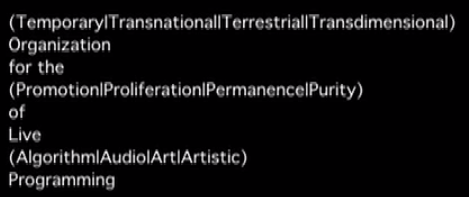
\includegraphics[scale=0.6]{imagens/TOPLAP.png}
  \caption{Definição do siginificado de TOPLAP. \textbf{Fonte}: \citeonline{ramsay_algorithms_2010}.}
  \label{fig:TOPLAP}
\end{figure}

O símbolo ``|'' é uma representação gráfica do operador lógico \emph{OR} (OU), bastante utilizado em algoritmos condicionais. Isto é, \emph{Temporary }| \emph{Trasnational} | \emph{Terrestrial} | \emph{Transdimensional} significa que as letras ímpares ``T'', e ``P'' e ``A'', podem significar um ou outro termo indicado pelo algoritmo.

Este comportamento, de permutar ordem das letras é praticado por Nick Collins (1975-); a permutação de suas letras é utilizada pelo pesquisador para gerar pseudônimos como Click Nilson, ou Sick Lincoln. Isso transparece uma técnica de uso frequente na improvisação de códigos, provavelmente pela facilidade de sua implementação computacional em amb. Por exemplo, o \emph{SuperCollider} oferece um método chamado \emph{scramble}, que embaralha a ordem de um conjunto (de caracteres). Mais especificamente, a permutação de letras transparece uma reorganização gramatica, mas que também reflete em técnicas de reorganização algorítmica da gramática musical.

\subsubsection{\emph{Show us your screens}}\label{sec:showusyourscreens}

Além das performances inaugurais nos festivais Europeus, o manifesto Lubeck04, \traducao{iniciado em um ônibus de trânsito Ryanair\disponivelem{https://www.ryanair.com/pt/pt/}, em  Hamburgo, para o aeroporto Lübeck\cite[p.~247]{ward_live_2004}}{begun on a Ryanair transit bus from Hamburg to Lubeck airport}, mais conhecido como ``\emph{Show us your screens}'', prescreve algumas regras práticas do \emph{live coding}. 

\begin{citacao}
Exigimos:

• Acesso à mente do intérprete, para todo o instrumento humano.

• Obscurantismo é perigoso. Mostre-nos suas telas.

• Programas são instrumentos que podem modificar eles mesmos.

• O programa será transcendido - Língua Artificial é o caminho.

• O código deve ser visto assim como ouvido, códigos subjacentes visualizados bem como seu resultado visual.

• Codificação ao vivo não é sobre ferramentas. Algoritmos são pensamentos. Motosserras são ferramentas. É por isso que às vezes algoritmos são mais difíceis de perceber do que motosserras.

Reconhecemos contínuos de interação e profundidade, mas preferimos:

• Introspecção dos algoritmos.

• A externalização hábil de algoritmo como exibição expressiva/impressiva de destreza mental.

• Sem \emph{backup} (minidisc, DVD, safety net computer).

Nós reconhecemos que:

• Não é necessário para uma audiência leiga compreender o código para apreciar, tal como não é necessário saber como tocar guitarra para apreciar uma performance de guitarra.

• Codificação ao vivo pode ser acompanhada por uma impressionante exibição de destreza manual e a glorificação da interface de digitação.

• Performance envolve contínuos de interação, cobrindo talvez o âmbito dos controles, no que diz respeito ao parâmetro espaço da obra de arte, ou conteúdo gestual, particularmente direcionado para o detalhe expressivo. Enquanto desvios na tradicional taxa de reflexos táteis da expressividade, na música instrumental, não são aproximadas no código, por que repetir o passado? Sem dúvida, a escrita de código e expressão do pensamento irá desenvolver suas próprias nuances e costumes. 
\footnote{\loccit{ward_live_2004}. Tradução nossa de:\emph{We demand: \begin{inparaenum}[•]
\item Give us access to the performer's mind, to the whole human instrument.
\item Obscurantism is dangerous. Show us your screens.
\item Programs are instruments that can change themselves.
\item The program is to be transcended - Artificial language is the way.
\item Code should be seen as well as heard, underlying algorithms viewed as well as their visual outcome.
\item Live coding is not about tools. Algorithms are thoughts. Chainsaws are tools. That's why algorithms are
sometimes harder to notice than chainsaws.
\end{inparaenum}. We recognise continuums of interaction and profundity, but prefer:  \begin{inparaenum}[•]
\item Insight into algorithms
\item The skillful extemporisation of algorithm as an expressive/impressive display of mental dexterity
\item No backup (minidisc, DVD, safety net computer)
\end{inparaenum}. We acknowledge that: \begin{inparaenum}[•]
\item It is not necessary for a lay audience to understand the code to appreciate it, much as it is not necessary
to know how to play guitar in order to appreciate watching a guitar performance.
\item Live coding may be accompanied by an impressive display of manual dexterity and the glorification of the
typing interface.
\item Performance involves continuums of interaction, covering perhaps the scope of controls with respect to
the parameter space of the artwork, or gestural content, particularly directness of expressive detail. Whilst
the traditional haptic rate timing deviations of expressivity in instrumental music are not approximated in
code, why repeat the past? No doubt the writing of code and expression of thought will develop its own
nuances and customs.
\end{inparaenum}}}
\end{citacao}

Escolhemos dois pontos de interesse ; as frase ``Obscurantismo é perigoso. Mostre-nos suas telas'' e  ``Algoritmos são pensamentos, motosserras são ferramentas'',  foi muito discutida no processo de qualificação desta tese. O primeiro questiona: é realmente necessário a projeção dos códigos para a questão da performance, do ponto de vista musical/cênico?

\subsubsection{Obscurantismo é perigoso, mostre-nos suas telas}\label{sec:obscurantismo}

O manifesto acima surgiu, entre outros motivos, como uma resposta ao artigo ``\emph{Using Contemporary Technology in Live Performance; the Dilemma of the Performer}'' \cite{schloss_dilemma_2003}. A crítica principal de \citeauthoronline{ward_live_2004} refere-se ao sétimo dos questionamentos sugeridos para uma performance de improvisação ao vivo com computadores. Isto é, em um contexto de embate acadêmico, o desafio colocado por \citeonline[p.~241]{schloss_dilemma_2003} foi um estímulo considerável para  emancipação da improvisação de códigos. É curioso notar que o problema e a intenção de Schloss eram opostas ao que foi proposto por \citeauthoronline{ward_live_2004}:


\begin{citacao}
\traducao{Para reiterar, agora que nós temos computadores rápidos o suficiente para execução ao vivo, nós temos novas possibilidades, e um novo problema. Do começo da evidência arqueológica da música até agora, música era tocada acusticamente, e sempre foi fisicamente evidente como o som era produzido; alí existia uma relação de proximiidade entre gesto e resultado. Agora nós não temos mais que seguir as leis da física (ultimamente temos, mas não nos termos do que o observador vê), uma vez que nós temos completo poder do computador como intérprete e intermediário entre nosso corpo físico e o som produzido. \textbf{Por esta causa, a ligação entre gesto e resultado foi completamente perdido, se é que existe ligação. Isto significa que nós podemos ir além da relação de causa-e-efeito entre executante e instrumento que faz a mágica.} Mágica é bom; muita mágica é fatal.}{
To reiterate, now that we have fast enough computers toperform live, we have new possibilities, and a new problem.From the beginning of the archeological evidence of musicuntil now, music was played acoustically, and thus it wasalways physically evident how the sound was produced; there was a nearly one-to-one relationship between gesture andresult. Now we don’t have to follow the laws of physicsanymore (ultimately we do, but not in terms of what theobserver observes), because we have the full power of computers as interpreter and intermediary between our physicalbody and the sound production. Because of this, the link between gesture and result can be completely lost, if indeed there is a link at all. This means that we can go so far beyond the usual cause-and-effect relationship between performer and instrument that it seems like magic. Magic is great; too much magic is fatal
} 
\end{citacao}

A crítica de \citeonline[p.~239]{schloss_dilemma_2003}: \traducao{considerar a visão do observador sobre os modos de performance das interações físicas e mapeamentos de gestos em som, para fazer uma performance convincente e efetiva}{Its now necessary, (\ldots) ;to consider the observer’s view of the performer’s modes of physical interactions and mappings from gesture to sound, in order to make the performance convincing and effective.} era especificamente direcionada aos compositores que improvisam música computacional no palco com foco apenas no aspecto sonoro ou tecnológico. Sua questão tange a ausência de gestos referenciais, esforço físico, no caso de performances com dispositivos extendidos, o problema do movimento exagerado, e a expectativa cênica na performance musical:


\begin{citacao}
\traducao{1. Causa-e-efeito é importante, pelo menos para o observador/audiência em uma sala de concerto. 
\ \\
2.Corolário: Mágica na performance é bom. Muita mágica é fatal! (chato).
\ \\
3. Um componente visual é essencial para a audiência, tal como existe um aparato visual de entrada para parâmetros e gestos.
\ \\
4. Sutileza é importante. Grandes gestos são facilmente visíveis de longe, o que é bom, mas eles são movimentos de desenho animado se comparados à execução de um instrumento musical.
\ \\
5. Esforço é importante. Neste sentido, nós estamos em desvantagem de desempenho na performance musical com o computador.
\ \\
6. Improvisação no palco é bom, mas ``mimar'' o aparato no palco não é improvisação, é edição. É provavelmente mais apropriado fazer isso no estúdio antes do concerto, ou se durante o concerto, com o console no meio ou atrás da sala de concerto.
\ \\
7. Pessoas que representam devem representar. Um concerto de música de computador não é uma desculpa/oportunidade para um programador(a) se sentar no palco. Sua presença melhora ou impede o desempenho da representação?
}{1. Cause-and-effect is important, at least for the observer/audience in a live concert venue. 2. Corollary: Magic in a performance is good. Too much magic is fatal! (Boring). 3. A visual component is essential to the audience, such that there is a visual display of input parameters/gestures. The gestural aspect of the sound becomes easier to experience. 4. Subtlety is important. Huge gestures are easily visible from far away, which is nice, but they are cartoon- movements compared to playi
ng a musical instrument. 5. Effort is important. In this regard, we are handicapped in computer music performance. 6. Improvisation on stage is good, but “baby-sitting” the apparatus on stage is not improvisation, it is editing. It is probably more appropriate to do this either in the studio before the concert, or if at the concert, then at the console in the middle or back of the concert hall. 7. People who perform should be performers. A computer music concert is not an excuse/opportunity for a computer programmer to finally be on stage. Does his/her presence enhance the performance or hinder it?} 
\end{citacao}

Duas opiniões divergentes resolvem seus problemas de maneiras divergentes sem considerarem como uma pode auxiliar a outra. No item 3, é apontado uma questão: para a audiência, e não para o improvisador, o componente visual é essencial (substantificação provável da prática). Ward et al. vão no caminho oposto ao de Schloss, e exageram este item, ao projetar códigos. Mas para Schloss, realizar isso é mimar o aparato (e o público), e tornar a apresentação pedante. É curioso notar, que Schloss faz um apontamento importante, no item 5, sobre a ausência de esforço. Não que ela seja premissa para o resultado sonoro. Mas para o público, e Schloss trata exatamente deste ponto na performance musical (item 1). Mas a crítica mais ácida é o item 7, cujo pensamento não difere de uma lógica fordiana: as atividades de artista e de programador devem ser bem definidas, e separadas. Para Schloss, são duas atividades que não se complementam. Para McLean, são interdisciplinares.


\subsubsection{Algorithms are Thoughts, Chainsaws are Tools}

``Algorithms are Thoughts, Chainsaws are Tools'' é o nome dado ao vídeo de Stephen \citeonline{ramsay_algorithms_2010}, publicado no Vimeo, em  27 de fevereiro de 2010, como um \emph{Coffee-Table Movie}. É uma análise pessoal da performance de \emph{Strange Places} de Andrew Sorensen. O nome do vídeo é derivado de uma das regras práticas apresentadas na \autoref{sec:showusyourscreens}, p. \pageref{sec:showusyourscreens}; mais especificamente, o sexto item.

O algoritmo como pensamento é um espaço conceitual abstrato \ver{cap:metodologia}; pode conter qualquer fundamento teórico pertinente para uma improvisação específica. O dispositivo usado (motoserra, máquina de tecelagem ou o computador) é um meio pelo qual uma estratégia transversal \ver{sec:imagem_mental} toma sua forma sonora. É interessante aqui notar que este vídeo contém uma descrição e comentários que podem elucidar a frase-alvo sob o prisma da partitura musical. Abaixo realizei uma compilação de fragmentos de alguns dos comentários que considerei pertinentes. Ramsey apresenta a seguinte descrição do vídeo:

\begin{citacao}
Um curta sobre \emph{livecoding} apresentado como parte do Grupo de Estudos de Crítica de Códigos, em 2010, por Stephen Ramsay. Apresenta uma leitura ao vivo $[$\emph{live reading}$]$ de uma performance do compositor Andrew Sorensen. Também fala sobre J.D. Salinger, the Rockets, tocando instrumentos, Lisp, do clima em Brisbane e tímpanos \footnote{\loccit{ramsay_algorithms_2010} Tradução de \emph{A short film on livecoding presented as part of the Critical Code Studies Working Group, March 2010, by Stephen Ramsay. Presents a "live reading" of a performance by composer Andrew Sorensen. It also talks about J. D. Salinger, the Rockettes, playing musical instruments, Lisp, the weather in Brisbane, and kettle drums.}.}.
\end{citacao}

Sem entrar em méritos críticos do registro, limitamo-nos a descrever como um VLog, uma variante no formato audiovisual de \emph{weblogs}\footnote{\cfcite{baker_origins_2008}.}. Se caracteriza por ser um vídeo de curta duração, com opiniões pessoais de quem fez, geralmente no quarto da pessoa, com \emph{headsets} (microfone+headphones). A prática de inserir comentários em um é bastante útil para levantar outras opiniões. Realizamos a tradução de alguns comentários. Não são nossas opiniões, mas podem oferecer ao leitor uma abrengência sobre o que pensam um público entusiasta.

Amanda French nega a utilização do termo \emph{partitura} para explicitar diferenças no uso da programação-partitura, em uma performance de improvisação com o computador, para uma performance não-improvisada com partitura.

\begin{citacao}
A noção de partitura não se aplica aqui, é como não fosse possível aplicá-lo ao músico de \emph{jazz} ou tocador de \emph{bluegrass}. (\ldots). Levanta a questão, para mim, se, em uma sessão de \emph{livecoding} *feita*, constite simplismente no ato de digitar em um programa existente, seria tão convincente -- eu acho que isso pode definitivamente ter pontos de interesse. Ou qual seria o análogo do \emph{livecoding} para uma performance não-improvisada de música?\footnote{\loccit{ramsay_algorithms_2010} Tradução parcial de \emph{The notion of "sheet music" doesn't apply here, as it wouldn't apply to a jazz musician or a bluegrass picker. Even the name of his environment, Impromptu, makes that point. Raises the question for me precisely of whether a livecoding session that *did* consist of simply typing in an existing program would be as compelling -- I think it would definitely have its points of interest, actually. Or what would the livecoding analog be to a non-improvisational live performance of music?}}
\end{citacao}

Um segundo comentário de Matt King, coloca a pergunta de Amanda em outra perspectiva:

\begin{citacao}
O que torna o \emph{livecoding} diferente, e pode a performance de música tradicional imitar isso? Para responder esta questão, parece importante notar que as formas nas quais a música improvisada muitas vezes apela para alguma noção de autenticidade ou gênio. Enquanto o \emph{livecoding} ele mesmo à noção de virtuosismo de código, ``autenticidade'' parece fora de lugar aqui. Se música improvisada sugere expressão, o \emph{livecoding} sugere um conjunto de restrições na expressão, descrevendo os parâmetros através dos quais a máquina $[$midi$]$ ganha expressão \footnote{Tradução nossa de \emph{(\ldots) What makes livecoding different, and can a traditional music performance mimic it? To answer this question, it seems important to note the ways in which improvised music often appeals to some notion of authenticity or genius. While livecoding might lend itself to some notion of coding virtuosity, "authenticity" seems out of place here. If improvised music is expression, livecoding suggests a setting of constraints on expression, describing the parameters through which the machine (midi) gets expressed.}}
\end{citacao}

Michel Pasin defende que o ato de improvisação musical requer conhecimentos técnicos prévios, mas não necessariamente correlacionados ao conhecimento do que é uma partitura: \traducao{Em geral, é somente dominando um instrumento que você pode esquecer sobre a técnica e concentrar em 'dizer' coisas com o instrumento.}{In general, it is only by mastering an instrument that you can forget about the technique and concentrate on 'saying' things with the instrument.}. Este caso é bastante específico de performances com linguagens de baixo e alto-nível. Porém seria possível objetar que a prática de construção de linguagens artificiais, no topo de outras linguagens artificiais, possibilita um praticante não-familiarizado com a programação elaborar rotinas computacionais.  Porém aí caímos em um problema: estaria o praticante realizando uma improvisação de códigos? ou melhor, isso importa, se o objetivo é a criação musical? Para delinear estas questões buscamos definir no próximo capítulo o que consideramos por objetivo de um agenciamento sonoro improvisado.

\section{Discussão}

Neste capítulo delimitamos a discussão musical afim de ilustrar a improvisação de códigos do ponto de vista de uma bricolagem conceitual. Exemplificamos a prática de improvisar códigos em situações onde é possível seguir dois caminhos para criar artefatos artísticos: o primeiro segue a trilha do formalismo, com concertos, espetáculos em teatros. O segundo ocorre informalmente, e geralmente está ligado à diversão, ou um encontro como uma oficina. Por outro lado, esta divisão binária pode expandir para áreas como tecelagem, dança e música. Não discutimos a situação audiovisual em seus detalhes, pois é um campo proeminente. Existem ainda as abordagens de instalações artísticas, jogos, e aplicações pedagógicas. Mas deixaremos a tarefa para quem se dispor. Ademais, oferecemos um cenário proto-histórico do ponto de vista, na Itália com o compositor Pietro Grossi, nos EUA com Jim Horton, John Bischoff, Tim Perkis, e na Holanda com Ron Kuivila (residente nos EUA), que deram suporte ao pensamento promovido na Inglaterra e Alemanha. Sugestões para essa proto-história foram colocados no \autoref{app:B}. Na 